%----------------------------------------------------------------------------------------
%	9./ Photometry&Stability
%----------------------------------------------------------------------------------------
%\section{Photometry \& Stability Assessment}
%\label{se:photometry}
%%----------------------------------------------------------------------------------------
%	9./ Photometry&Stability
%----------------------------------------------------------------------------------------
%\section{Photometry \& Stability Assessment}
%\label{se:photometry}
%%----------------------------------------------------------------------------------------
%	9./ Photometry&Stability
%----------------------------------------------------------------------------------------
%\section{Photometry \& Stability Assessment}
%\label{se:photometry}
%%----------------------------------------------------------------------------------------
%	9./ Photometry&Stability
%----------------------------------------------------------------------------------------
%\section{Photometry \& Stability Assessment}
%\label{se:photometry}
%\input{Photometry.tex}

NIKA2 photometric capabilities after the calibration presented in
Sect.~\ref{se:calibration}, are assessed in this section. Firstly,
we use observation of secondary calibrators (planetary nebulae NGC7027, CRL2688, and
MWC349A) to test the consistency of the flux density estimates with
expectations. The flux density expectations
in NIKA2 bands for these calibrators are given in
Appendix~\ref{se:ref_flux_secondaries}. Then,
we verify the stability of the photometry with
respect to the atmospheric conditions using a large amount of
observations toward a large variety of sources. 

The quality criteria used to assess the photometric
capabilities and calibration results are defined in
Sect.~\ref{se:photometry_criteria}.
In Sect.~\ref{se:photometry_baseline}, these criteria are evaluated
for the baseline calibration, and in Sect.~\ref{se:photometry_others},
we compare these results with other calibration method results. 


%---------------------------------------------------------------------
%	Criteria
%---------------------------------------------------------------------
\subsection{Calibration accuracy and uncertainty assessment}
\label{se:photometry_criteria}

We assess the photometric performance by evaluating two
quality criteria: first, the calibration bias checks the accuracy of
the absolute calibration and then the calibration relative
uncertainties test the stability of the flux densities. \\

\noindent \emph{Calibration bias} We define the calibration bias
$b_{\nu}$, where $\nu$ stands for Array 1, 2, 3 and the
$1\,\rm{mm}$ array combination, as
the ratio between the measured flux density $\hat{S}_{\nu}$ using the
%fixed-width Gaussian beam
reference photometry
(Sect.~\ref{se:photometric_system}) and the flux density
expectations $S_{\rm{s}}(\nu_0)$ as given in
Appendix~\ref{se:ref_flux_secondaries}. From a series of
secondary calibrator scans, we evaluate the average calibration bias
$b_{\nu}$, which by construction, should be equal to
unity within uncertainties.
%the precision with which the expected flux densities are known.
Moreover, we check the stability of the calibration bias against
the observed opacities as a robustness test of the
opacity derivation method. Likewise, we verify that the photometry is
insensitive to optical variations by checking the stability of the
calibration bias against the measured beam size.\\

\noindent \emph{Calibration uncertainties} We evaluate the standard
deviation of bright source measured-to-median flux density ratio
$\sigma_{\nu}$ per array or array combination $\nu$. {\lp Since the flux
density ratios are not Gaussian distributed, we
evaluate the 68 and 95\% confidence level (C.L.) contours using the
measured distributions in order to further characterise the
uncertainties. We check that the rms
errors are larger than the 68\% C.L. contours and thus provide
conservative $1\sigma$-like errors.}    

As the flux density of most of the considered sources is unknown a priori, we
compare the flux density estimate in a single observation scan to the
average flux density throughout an observation campaign. This method
requires the selection of sources that are bright enough to be detected with a high
signal-to-noise ratio with a single repetition of an usual
$8'\times 5'$ OTF raster scan. Namely, we perform a source
selection by thresholding the flux estimate to $800\,\rm{mJy}$ at
$1\,\rm{mm}$ and $400\,\rm{mJy}$ at $2\,\rm{mm}$. Moreover, we consider
only the sources for which a minimum of $10$ scans are available after
selection to ensure a precise average flux density
estimation. Finally, the selected source scans must meet the \emph{baseline}
scan selection criteria given in Sect.~\ref{se:data_selection}.

{\lp As the rms of the flux density ratio is estimated on a scan set
that is representative of the observing conditions encountered at
the \trentemetre\ telescope, this is an estimate of the
calibration uncertainties that encloses errors of
optical, atmospheric, instrumental noise and data processing
origins. This includes the errors sourced by the \afternoon\ beam 
variations, the effect of the elevation, the uncertainties of the
atmospheric opacity correction using either the {\tt skydip} or
the {\tt taumeter} method and the atmospheric and instrumental noise
residuals after the data reduction (Sect.~\ref{se:dataproc}).

To obtain an estimate of the total absolute
calibration uncertainties, the rms errors must be added in quadrature
with systematic uncertainties that do not depend on the observing
conditions. The main source of systematic error is the model uncertainty
on the primary calibrator flux density expectations. In the case of
Uranus, \citet{Morenothesis} and \citet{Bendo2013} report model
uncertainties of about $5\%$ at both wavelenghts.

When using the \emph{baseline}
calibration method, which resorts to the {\tt corrected skydip} method
for the atmospheric opacity correction (see
Sect.~\ref{se:corrected-skydip}), the uncertainties on the
correcting factor $a_\nu^{\rm{skydip}}$, as defined in
Eq.~\ref{eq:corrected_skydip}, must be propagated to the flux
uncertainties. These uncertainties, which are referred to as the
{\tt corrected skydip} uncertainties, depend on the line-of-sight atmospheric
opacity $\taunu x$. Precisely, because the {\tt corrected skydip}
opacity correction is consistently used for both the primary
calibrator and the target source flux measurement, the {\tt corrected skydip}
uncertainties depends on the difference between the average
line-of-sight opacity of the primary calibrator scans and the
line-of-sight opacity of the source scan.   
We evaluate the {\tt corrected skydip} uncertainties for two
different $\taunu x$ values. First for the reference IRAM \trentemetre\
winter observing conditions, as defined as $2\,\rm{mm}$ of pwv and an
elevation of $60^{\rm{o}}$, the {\tt corrected skydip} uncertainties are of
0.6\% at $1\,\rm{mm}$ and 0.3\% at $2\,\rm{mm}$. Secondly in the worst
observing conditions allowed by the \emph{baseline} scan selection,
which are $\taunu x$ of 0.7 at $1\,\rm{mm}$ and of 0.5 at
$2\,\rm{mm}$, we find {\tt corrected skydip} uncertainties of 2\% and
$1.5\%$ at 1 and $2\,\rm{mm}$, respectively. These constitute
conservative upper limits on the {\tt corrected skydip}
uncertainties.

The uncertainties on NIKA2 bandpass measurements (see
Sect.~\ref{se:instru_bandpass}) propagate into
uncertainties on the flux densities after the color correction using
Eq.~\ref{eq:color_correction}. These
uncertainties depend on the source SED but are neglectible in most of
the cases. In particular, for MWC349, we find uncertainties below 0.1\% at
both wavelengths.}





%---------------------------------------------------------------------
%	Baseline results
%---------------------------------------------------------------------
\subsection{Baseline calibration photometry results}
\label{se:photometry_baseline}

We measure the calibration bias and statistical uncertainties, as defined
in the previous section (Sect.~\ref{se:photometry_criteria}) using the
\emph{baseline} calibration method (Sect.~\ref{se:baseline_calibration}).

%  BASELINE RESULTS
%%%%%%%%%%%%%%%%%%%%%%%%%%%%%%%%%%%%%%%%%%%%%%%%%%%%%%%%%%%%%%%%%%
\begin{table}[!thbp]
  \begin{center}
    \caption[Baseline calibration results]{Baseline calibration results:
  photometry accuracy and uncertainties. The first subpanel labelled 'Bias' gives the
  calibration bias $b_{\nu}$ and the second subpanel labelled 'Rms' the calibration
  rms error $\sigma_{\nu}$, as defined in
  Sect.~\ref{se:photometry_criteria},
  using observations during N2R9, N2R12, N2R14 and the combination of
  the three campaigns. {\lp In each subpanel, the first row indicates the
    number of acquired scans, while the second row gives the
    number of selected scans using the \emph{baseline} scan selection.}}
\label{tab:baseline-photometry}
\begin{tabular}{clrrrr}
  \hline\hline
  \noalign{\smallskip}
 % \multicolumn{2}{c}{}  &  \multicolumn{4}{|c}{Datasets}  \\\cline{3-6}
  \multicolumn{2}{c}{Characteristics} &  N2R9  & N2R12   &  N2R14 & Combined \\
  \noalign{\smallskip}
  \hline
  \noalign{\smallskip}
%  Bias &  $\#$ total    &  68    &  14     &   27     &    109    \\
%       &  $\#$ selected &  64    &   1     &   7      &     72    \\
%       &  A1            &  0.99  &  1.06   &   0.98   &   0.98    \\
%       &  A3            &  1.01  &  1.08   &   1.04   &   1.00    \\
%       &  1mm           &  1.00  &  1.07   &   1.01   &   0.99    \\
%       &  2mm           &  0.95  &  0.96   &   0.94   &   0.95    \\
%  \hline
%  \multicolumn{6}{|l|}{using color corrections as of Table A.1}  \\
%  \hline
  Bias &  $\#$ total    &  68    &  14     &   27     &    109    \\
       &  $\#$ selected &  64    &   1     &   7      &     72    \\
       &  A1            &  0.95  &  1.03   &   0.94   &   0.95    \\
       &  A3            &  0.99  &  1.07   &   1.00   &   1.00    \\
       &  1mm           &  0.97  &  1.05   &   0.97   &   0.98    \\
       &  2mm           &  0.95  &  0.95   &   0.93   &   0.95    \\
  \hline
  \noalign{\smallskip}
  Rms  &  $\#$ total    &  303   &  72     &   112    &    487   \\
  $[\%]$ &  $\#$ selected &  219   &  33     &    12    &    264   \\
       &  A1            &  5.7   &  4.6    &   2.9    &    5.5   \\
       &  A3            &  6.2   &  5.7    &   2.4    &    6.0   \\
       &  1mm           &  5.9   &  5.0    &   2.5    &    5.7   \\
       &  2mm           &  3.2   &  2.1    &   1.1    &    3.0   \\  
\hline
\end{tabular}
\end{center}
\end{table}

The calibration bias is evaluated using a
series of scans of MWC349 acquired during the
%N2R9, N2R12 and N2R14
 reference observation campaigns. Namely, we use the 72 scans that met
 the \emph{baseline} selection
 criteria (see Sect.~\ref{se:data_selection}) over the 109 available
scans for MWC349. The first row of
Fig.~\ref{fig:mwc349_obstau_others}, labelled 'baseline', shows the
calibration bias $b_{\nu}$ for the combination of the $1\,\rm{mm}$ arrays and
Array 2 as a function of the atmospheric transmission %, which is
%evaluated with the zenith opacity $\taunu$ and the airmass $x$ as
$\exp \left( - \taunu \, x \right)$. No significant dependency of the
calibration bias on the atmospheric transmission is observed. 

Table~\ref{tab:baseline-photometry} gathers the calibration bias
estimates for the three observation campaigns and for all the scans.
In the $1\,\rm{mm}$ band, we find
$b_\nu$ in agreement with unity within the statistical dispersion for
the three campaigns,
whereas a $5\%$ lack of flux with respect to expectations is observed
at $2\,\rm{mm}$, consistently for the three campaigns. This bias has a
low significance with respect to the absolute calibration precision of
NIKA2 (see Sect.~\ref{se:photometry_criteria}).
%{\lp Furthermore, the flux density expectations have also
%uncertainties.}
%and PdBI, which depend on the precicision with which the
%primary calibrator flux densities are known. For Uranus, the model
%uncertainties are of about $5\%$, as reported
%in~\citet{Morenothesis,Bendo2013}. 
This will be further investigated by using other calibration methods
in Sect.~\ref{se:photometry_others}.


%The baseline calibration relative uncertaintes, as defined in
%Sect.~\ref{se:photometry_criteria}, are evaluated using bright
%sources. From a total of 487 scans
%flux-selected sources acquired during N2R9, N2R12 and N2R14, 264 met
%the baseline selection criteria and are used for testing stability.
Figure~\ref{fig:allbright_rms_corrected_skydip} shows the
measured-to-median flux densities evaluated from bright source scans
for the combination of Array $1\&3$ and Array 2 as a function of the
atmospheric transmission and color-coded as a function of the
observation time. From a total of 487 scans towards
flux-selected sources, acquired during N2R9, N2R12 and N2R14, 264 met
the baseline selection criteria and are included in
Fig.~\ref{fig:allbright_rms_corrected_skydip} for testing the
calibration stability. The statistical calibration uncertainties are
estimated using the standard deviation of the flux density ratios for
the three campaigns. Results are gathered in
Table~\ref{tab:baseline-photometry}.
Combining all the scans, we find uncertainties of $5.5\%$ for A1,
$6.0\%$ for A3, $5.7\%$ for the $1\,\rm{mm}$ band and $3.0\%$ for A2.
%%%%%%% 95% %%%%%%%%%%%%%%%%%%%%%%%%
{\lp Using the flux ratio distributions, we construct the 68 and 95\%
C.L. intervals. The 68\% C.L. intervals are $-6.4\%$ and $+3.4\%$ at
$1\,\rm{mm}$ and $-3.8\%$ and $+1.5\%$ at $2\, \rm{mm}$. Hence in average
the 68\% C. L. errors are of $4.9\%$ and $2.7\%$ at 1 and $2\, \rm{mm}$,
respectively. We conclude that the rms errors are conservative
estimates of the 68\% C. L. errors at both wavelengths. The 95\%
C.L. contours are $-15.8\%$ and $+5.9\%$ at $1\,\rm{mm}$ and $-8.6\%$ and
$+3.8\%$ at $2\, \rm{mm}$.
The rms errors and the 95\%
C.L. interval are shown in
Fig.~\ref{fig:allbright_rms_corrected_skydip} with the inner and
outter dashed lines, respectively.} 


The flux density ratio is constant within the rms errors along the
wide range of tested atmospheric transmission, ranging from 0.5 to 0.9
at $1\,\rm{mm}$.
However, some scans at atmospheric transmissions of about 0.7 at
$1\,\rm{mm}$ show a mild lack of flux density with respect to the
median within the 95\% C. L. contours. The scans
affected by the lack of flux have all been observed
either between 12:00 and 14:00 UT or between 8:00 and 9:00 UT,
that are close to the threshold of the observation time cuts of
the \emph{baseline} scan selection (see
Sect.~\ref{se:data_selection}). These scans are likely
to be affected by the \afternoon\ beam broadening or by the
sunrise focus drift, respectively. Furthermore, we find that restricting the
used observation time to the 10 more stable hours (from 22:00 to
08:00 UT) would result in rms calibration uncertainties of
$3.6\%$ at $1\,\rm{mm}$ and $1.2\%$ at $2\,\rm{mm}$, which constitute an
improvement of about $60\%$ at $1\,\rm{mm}$ and $40\%$ at $2\,\rm{mm}$
of the rms errors.  
The \emph{baseline} scan selection, which i)
retains 16 hours of observation time
a day and ii) %results in calibration uncertainties that meet the
%requirement for a millimetric ground-based instrument,
{\lp results in state-of-the-art statistical calibration
uncertainties,} constitutes an advantageous tradeoff.

%%%%%%%%%%%%%%%%%%%%%%%%%%%%%%%%%%%%%%%%%%%%%%%%%%%%%%%%%%%%%%%%%%%%%%%%%%%%%%%%%%%%%%%%%%%%%
%                              bias
\begin{figure}[!thbp]
  \begin{center}
    \begin{overpic}[clip=true, trim={0.9cm, 0.2cm, 0, 0.6cm},width=0.532\linewidth]{Figures/plot_flux_density_ratio_MWC349_obstau_corrected_skydip_narrow_1mm.pdf}
      \put(20,60){\footnotesize Baseline}
    \end{overpic}
    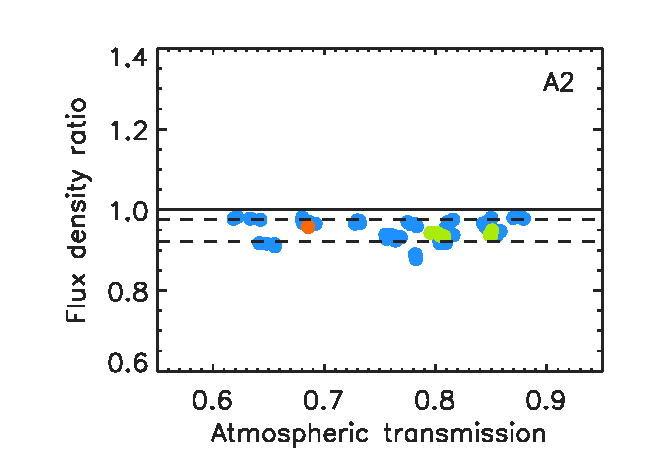
\includegraphics[clip=true, trim={1.8cm, 0.2cm, 0.5cm, 0.7cm},width=0.457\linewidth]{Figures/plot_flux_density_ratio_MWC349_obstau_corrected_skydip_narrow_a2.pdf}
    \begin{overpic}[clip=true, trim={0.9cm, 0.2cm, 0, 0.6cm},width=0.532\linewidth]{Figures/plot_flux_density_ratio_MWC349_obstau_tau225_narrow_1mm.pdf}
      \put(20,60){\footnotesize Taumeter}
    \end{overpic}
    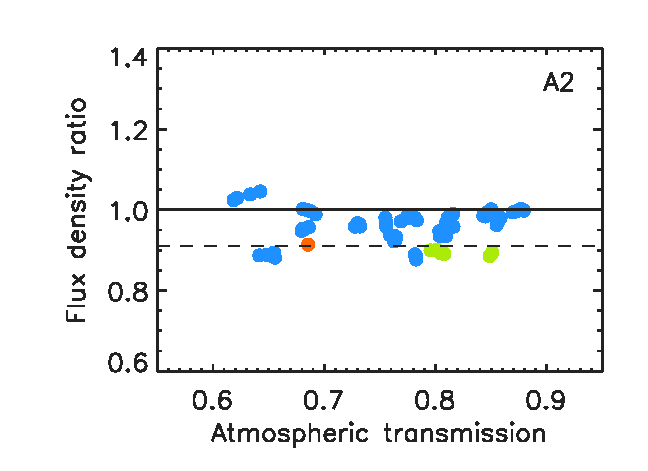
\includegraphics[clip=true, trim={1.8cm, 0.2cm, 0.5cm, 0.7cm},width=0.457\linewidth]{Figures/plot_flux_density_ratio_MWC349_obstau_tau225_narrow_a2.pdf}
    \begin{overpic}[clip=true, trim={0.9cm, 0.2cm, 0, 0.6cm},width=0.532\linewidth]{Figures/plot_flux_density_ratio_MWC349_obstau_skydip_narrow_1mm.pdf}
      \put(20,60){\footnotesize Skydip}
    \end{overpic}
    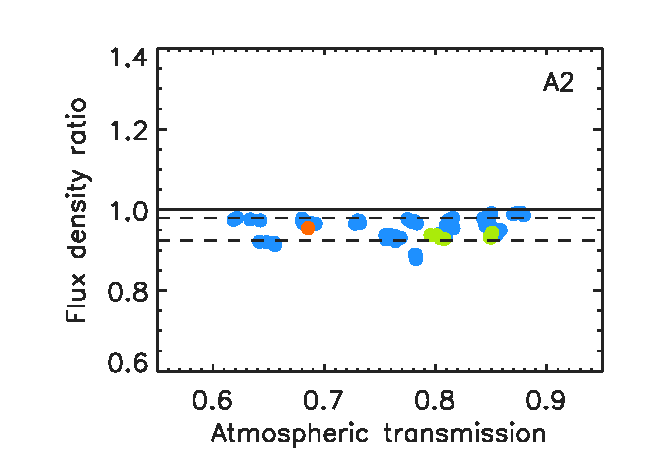
\includegraphics[clip=true, trim={1.8cm, 0.2cm, 0.5cm, 0.7cm},width=0.457\linewidth]{Figures/plot_flux_density_ratio_MWC349_obstau_skydip_narrow_a2.pdf}
    \begin{overpic}[clip=true, trim={0.9cm, 0.2cm, 0, 0.6cm},width=0.532\linewidth]{Figures/plot_flux_density_ratio_MWC349_obstau_corrected_skydip_photocorr_demo_narrow_1mm.pdf}
      \put(20,60){\footnotesize Photocorr Demo}
    \end{overpic}
    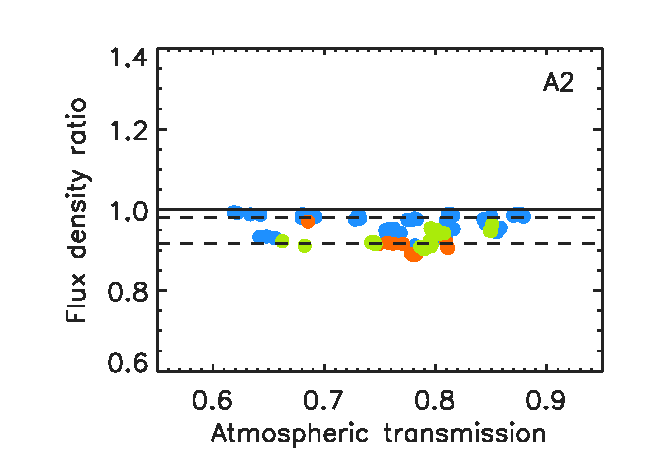
\includegraphics[clip=true, trim={1.8cm, 0.2cm, 0.5cm, 0.7cm},width=0.457\linewidth]{Figures/plot_flux_density_ratio_MWC349_obstau_corrected_skydip_photocorr_demo_narrow_a2.pdf}
    \begin{overpic}[clip=true, trim={0.9cm, 0.4cm, 0, 0.6cm},width=0.532\linewidth]{Figures/plot_flux_density_ratio_MWC349_obstau_corrected_skydip_photocorr_pointing_narrow_1mm.pdf}
      \put(20,60){\footnotesize Photocorr Pointing}
    \end{overpic}
    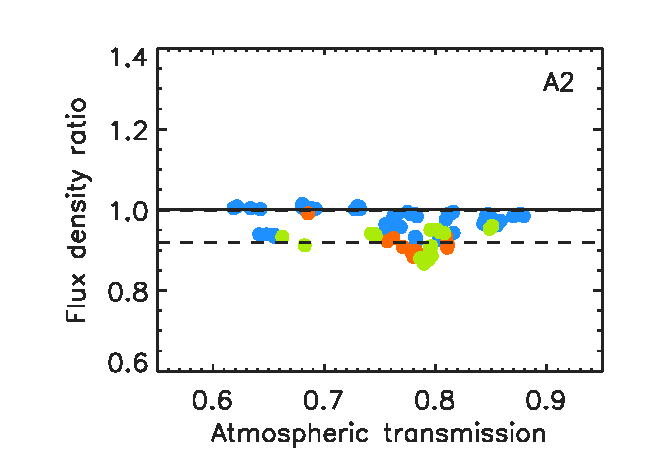
\includegraphics[clip=true, trim={1.8cm, 0.4cm, 0.5cm, 0.7cm},width=0.457\linewidth]{Figures/plot_flux_density_ratio_MWC349_obstau_corrected_skydip_photocorr_pointing_narrow_a2.pdf}
    \vspace{-0.3cm}
    \caption[Calibration bias comparison]{Comparison of the
        calibration bias for five calibration methods using
          observations of MWC349.
       The measured-to-expected flux density ratio is shown as a
      function of the atmospheric transmission for the baseline method
      (first row) as well as for methods using the {\tt taumeter} (second
      row) and {\tt skydip} (third) opacity correction, and for methods
      resorting to the {\tt PC-demo} (fourth) and {\tt PC-point} (fifth)
      photometric correction. Dashed lines
      show the flux density ratio $1 \sigma $ dispersion.}
    \label{fig:mwc349_obstau_others}
  \end{center}
\end{figure}

%
\begin{figure}[!thbp]
  \begin{center}
%    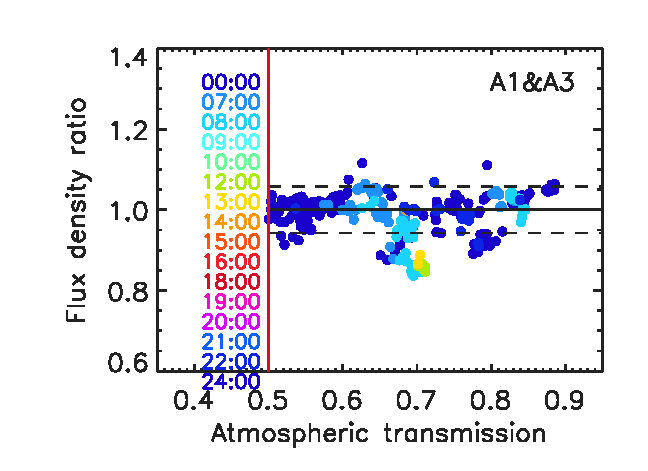
\includegraphics[clip=true, trim={0.9cm, 0.2cm, 0, 0.7cm},width=0.532\linewidth]{Figures/plot_flux_density_ratio_obstau_allbright_obsdate_corrected_skydip_narrow_1mm.pdf}
%    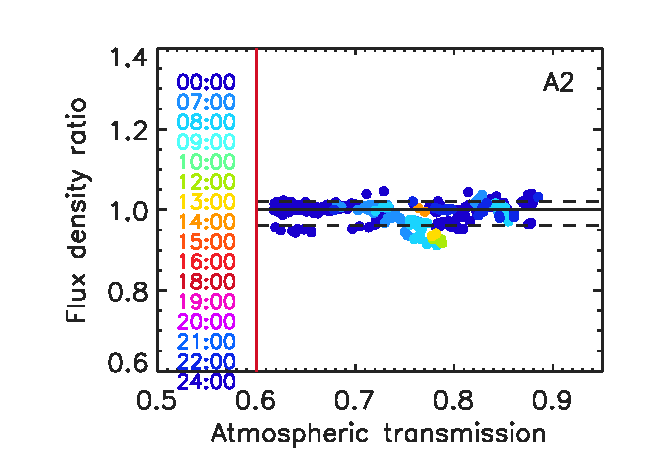
\includegraphics[clip=true, trim={1.8cm, 0.2cm, 0.5cm, 0.7cm},width=0.455\linewidth]{Figures/plot_flux_density_ratio_obstau_allbright_obsdate_corrected_skydip_narrow_a2.pdf}
%    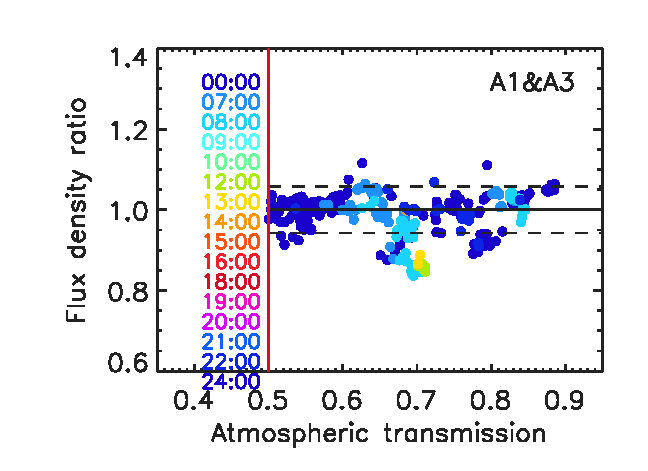
\includegraphics[clip=true, trim={0.9cm, 0.2cm, 0.5cm, 0.7cm},width=0.65\linewidth]{Figures/plot_flux_density_ratio_obstau_allbright_obsdate_corrected_skydip_narrow_1mm.pdf}
%     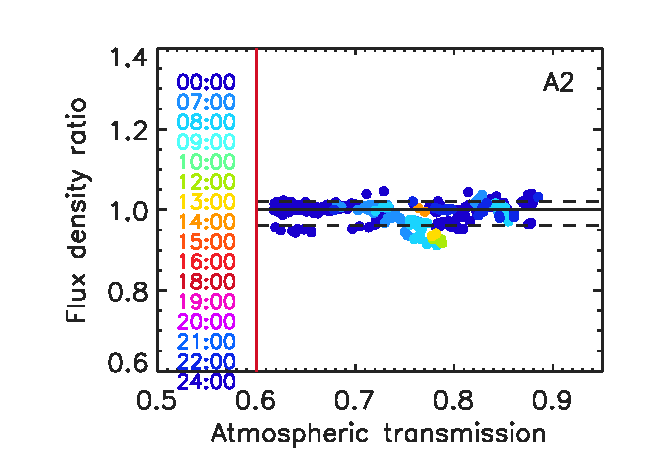
\includegraphics[clip=true, trim={0.9cm, 0.2cm, 0.5cm, 0.7cm},width=0.65\linewidth]{Figures/plot_flux_density_ratio_obstau_allbright_obsdate_corrected_skydip_narrow_a2.pdf}
      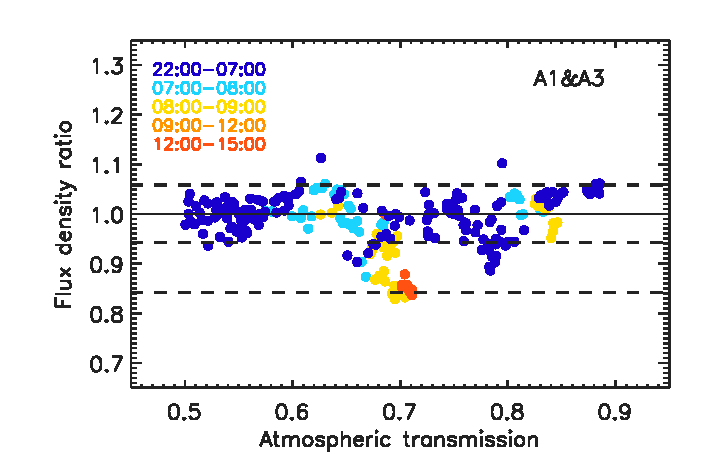
\includegraphics[clip=true, trim={0.9cm, 0, 0.5cm, 0.6cm},width=0.75\linewidth]{Figures/plot_flux_density_ratio_obstau_allbright_obsdate_corrected_skydip_rescaled_1mm.pdf}
     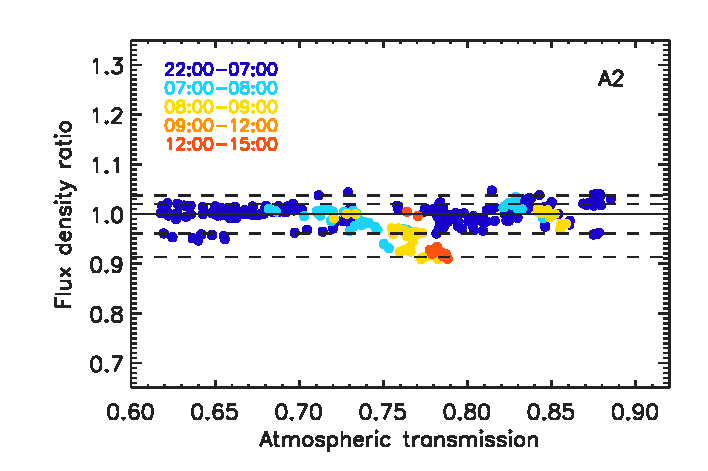
\includegraphics[clip=true, trim={0.9cm, 0, 0.5cm, 0.6cm},width=0.75\linewidth]{Figures/plot_flux_density_ratio_obstau_allbright_obsdate_corrected_skydip_rescaled_a2.pdf} 


    \caption[Baseline calibration rms error estimate]{Baseline
      calibration uncertainties. The
      measured-to-median flux density ratio of bright sources is
      plotted as a function of the atmospheric transmission
      color-coded according to the UT
      observation time of the scans for the combination of A1$\&$A3
      (top pannel)
      and for A2 (bottom pannel).
      The inner dashed lines from either sides of the
      unity-ratio line show the rms errors, {\lp which
      are less than 6\% at $1\,\rm{mm}$ and 3\% at $2\,\rm{mm}$, while
      the outer dashed lines show the $95\%$ confidence level contours.}
      The lowest flux ratio data points correspond to some of the
      scans acquired during daytime between 8:00 UT and 15:00 UT
      hours (yellow and red), while the scans acquired during nightime
      between 22:00 UT and 7:00 UT yield data points (dark blue)
      well distributed within the rms error with a few outliers.}
    \label{fig:allbright_rms_corrected_skydip}
  \end{center}
\end{figure}




%---------------------------------------------------------------------
%	Comparaison
%---------------------------------------------------------------------
\subsection{Comparison with other calibration methods}
\label{se:photometry_others}

% ALL METHOD RESULTS 
\begin{table*}[!htbp]
\begin{center}
\begin{tabular}{clrrrrr}
  \hline\hline
  \noalign{\smallskip}
  \multicolumn{2}{c}{}  &  \multicolumn{5}{c}{Methods} \\\cline{3-7}
  \noalign{\smallskip}
  \multicolumn{2}{c}{Characteristics} &  baseline  & {\small {\tt taumeter}}  & {\small {\tt skydip}}  &  {\small {\tt PC-demo}} & {\small {\tt PC-point}} \\
  \hline
  \noalign{\smallskip}
  %Bias &  $\#$ total    &   109   &   109    &   109    &    109    &  109   \\
  %     &  $\#$ selected &    72   &   72     &    72    &     96    &   95   \\
  %     &  A1            &   0.98  &  1.01    &  0.99    &   0.98    &  1.00  \\
  %     &  A3            &   1.00  &  1.04    &  1.01    &   1.01    &  1.02  \\
  %     &  1mm           &   1.00  &  1.03    &  1.00    &   1.00    &  1.01  \\
  %     &  2mm           &   0.95  &  0.96    &  0.95    &   0.95    &  0.95  \\
  %\hline
  %\multicolumn{7}{|l|}{Using color corrections as of Table A.1} \\
  %\hline
  Bias &  A1            &   0.95   &  0.98    &  0.97    &   0.95    &  0.97  \\
       &  A3            &   1.00   &  1.02    &  1.02    &   0.99    &  1.00  \\
       &  1mm           &   0.98   &  1.01    &  1.00    &   0.97    &  0.99  \\
       &  2mm           &   0.95   &  0.95    &  0.95    &   0.95    &  0.95  \\
  \hline
  \noalign{\smallskip}
  Rms  &  $\#$ total    &   487    &    487   &    487    &    396    &  396 \\
  $[\%]$ &  $\#$ selected &   264    &    264   &    264    &    291    &  283 \\
       &  A1            &   5.5    &    7.5   &    7.3    &    4.0    &  4.9 \\
       &  A3            &   6.0    &    8.1   &    7.1    &    4.1    &  5.2 \\
       &  1mm           &   5.7    &    7.9   &    7.1    &    3.8    &  4.9 \\
       &  2mm           &   3.0    &    3.8   &    3.0    &    2.2    &  2.4 \\
\hline
\end{tabular}
\caption[Comparison of calibration results using five
  methods]{Comparison of results using five calibration methods.}
\label{tab:Calibration_results_all}
\end{center}
\end{table*}

In this section, the \emph{baseline} calibration results are compared to
results drawn either using other calibration methods obtained from different
opacity corrections ({\tt taumeter} and {\tt skydip} as
discussed in Sect.~\ref{se:baseline_calibration_opacity}), or
including a photometric correction ({\tt PC-demo} and {\tt PC-point},
as described in Sect.~\ref{se:photometric_correction}). For robustness test, we
evaluate and compare the photometry quality critera of
Sect.~\ref{se:photometry_criteria} for the five calibration methods.


\subsubsection{Calibration bias}
\label{se:calibration_bias_all}

We present the calibration bias as a function of the atmospheric
transmission for the five calibration methods in
Fig.~\ref{fig:mwc349_obstau_others} and report the results in the row
labelled 'Bias' of Table~\ref{tab:Calibration_results_all}.

At $1\,\rm{mm}$, all methods lead to flux density estimates in
agreement with expectations within the rms dispersion. However,
{\tt taumeter} flux ratios have more dispersion than
the \emph{baseline} flux ratios whereas {\tt skydip} shows some
dependency on the atmospheric
transmission, with a 10 to $15\%$ excess of the flux density with
respect to expectations at high transmission. Indeed this residual
systematic effect has motivated the development of the {\tt corrected
  skydip} method, as discussed in
Sect.~\ref{se:corrected-skydip}. These features, which are
already noticeable from Fig.~\ref{fig:mwc349_obstau_others}, will be
confirmed and further discussed later using more observation scans. On
the other hand, the calibration methods based on photometric
correction (Sect.~\ref{se:photometric_correction}) yield an
unbiased photometry (calibration bias in agreement with unity
within the rms error) while allowing the use of $30\%$ more
scans. These results are encouraging for the exploitation of scans
acquired during the observing periods
impacted by the \afternoon\ beam variation effect
(Sect.~\ref{se:beam_variation}).

At $2\,\rm{mm}$, all methods result in a similar calibration bias
of $0.95 \pm 0.05$, which corresponds to a low-significance $5\%$
lack of flux density toward MWC349.
%We also obtained the same calibration
%biases for each observation campaign (see
%Table~\ref{tab:baseline-photometry}).
To summarize, the calibration bias at $2\, \rm{mm}$ is stable against
i) a large range of atmospheric conditions, ii) the observation campaign, iii) the
opacity correction method, iv) the method to treat the
temperature-induced beam variation effect.
%An explanation for the
%$5\%$ lack of flux density toward
%MWC349 is probably to be seeked on the side of the flux density
%expectations for this source.
This $5\%$ lack of flux density is thus probably due to
uncertainties on the flux density expectations for this source.
They come in two flavours.
{\lp Firstly the uncertainties on the flux expectation, as reported in
Appendix~\ref{se:ref_flux_secondaries}, consist in the propagation of
the errors on the fitted SED from PdBI and VLA observations. Systematic
uncertainties that may also impact the SED are not included.}  
%the accuracy of the SED fitted from PdBI and VLA observations
%(see Sect.~\ref{se:ref_flux_secondaries})
%depends on these instruments absolute flux density calibration, which
%is at least greater than the $5\%$ primary calibrator model accuracy,
Secondly, the NIKA2 flux density extrapolation from
interferometer data may be not straightforward for MWC349. {\lp In
particular, NIKA2 flux extrapolation ignores the contamination by
strong masers in the radio recombination lines~\citep{masingRRL},
while strong maser emission lines are masked in PdBI observations to
measure the continuum. In addition, the resulting continuum shows
indications of variability.}


\subsubsection{Calibration uncertainties}

The calibration uncertainties for the five methods evaluated using
flux-selected source scans are gathered in the subpanel labelled 'Rms'
of Table~\ref{tab:Calibration_results_all}.

Compared to the baseline method, the {\tt taumeter} method leads to 
statistical uncertainty increased of about $40$ and $30\%$ at 1 and
$2\,\rm{mm}$. The {\tt skydip} method shows lower dispersion but a
mild correlation with the atmospheric transmission, as
discussed in Sect.~\ref{se:calibration_bias_all}.

In addition, we have checked the flux density ratios for the bunch of
scans with an atmospheric transmission of about 0.7, which were
discussed in Sect.~\ref{se:photometry_baseline}, by comparing
calibration methods with or without photometry correction. Whereas the
flux density ratios are low for the scans observed within 12:00 and
15:00 UT in the three first
methods, they are within the 68\% C.L. interval when using a photometric
correction. This further validates the hypothesis that the low flux
density of these scans is due to \afternoon\ beam effect, as assumed in
Sect.~\ref{se:photometry_baseline}. This also constitutes an example
of the calibration improvement obtained from resorting to a
photometric correction.

Moreover, results based on the {\tt PC-demo} method show that rms calibration
uncertainties as low as $3.8$ and $2.2\%$
at 1 and $2\,\rm{mm}$ are within the reach of NIKA2 {\lp without any
selection based on the observation time.}
%without rejecting any observations.
However, we recall this method relies on 
accurate beam estimates. Using {\tt PC-point}, which is the
practical case, still improves the calibration uncertainties
w.r.t. the baseline results but by a factor of about $20\%$ in both
bands. However, the differences between
the flux density ratios from {\tt PC-demo} and {\tt PC-point}, which are
seen e.g. from the 'photocorr demo' and 'photocorr pointing' of
Fig.~\ref{fig:mwc349_obstau_others}, are likely
to be due to the photometry correction noise
when monitoring the beam from pointing scans. We conclude that more
control on the beam monitoring is needed before routinely using a calibration
based on photometry correction. By contast, the baseline method
combines good performance with robustness.


\paragraph{Summary} Among the methods that rely on the UT hour-based
scan selection to mitigate the effect of beam size variations, the
baseline method shows the best performance in terms of calibration
bias and uncertainties. The methods that rely on a photometric correction
lead to good calibration results, and thus represent a promising lead
to further improve the calibration uncertainties. However, their
robustness depends on the accuracy of the beam monitoring. {\lp The
proposed beam monitoring based on {\tt pointing} scans induces some
extra dispersion of the flux densities. A more accurate beam monitoring is
feasable but requires using dedicated observation scans.} 
Using the baseline method, the measured flux density of
MWC349 is in agreement with expectations within $5\%$ for both
wavelengths. Moreover, we find calibration uncertainties of $5.7\%$ at
$1\,\rm{mm}$ and $3\%$ at $2\,\rm{mm}$ using a series of 264 scans of
sources of flux density above $1\, \rm{Jy}/\rm{beam}$. These results
demonstrate the excellent accuracy and stability of the NIKA2
photometric capabilities.







NIKA2 photometric capabilities after the calibration presented in
Sect.~\ref{se:calibration}, are assessed in this section. Firstly,
we use observation of secondary calibrators (planetary nebulae NGC7027, CRL2688, and
MWC349A) to test the consistency of the flux density estimates with
expectations. The flux density expectations
in NIKA2 bands for these calibrators are given in
Appendix~\ref{se:ref_flux_secondaries}. Then,
we verify the stability of the photometry with
respect to the atmospheric conditions using a large amount of
observations toward a large variety of sources. 

The quality criteria used to assess the photometric
capabilities and calibration results are defined in
Sect.~\ref{se:photometry_criteria}.
In Sect.~\ref{se:photometry_baseline}, these criteria are evaluated
for the baseline calibration, and in Sect.~\ref{se:photometry_others},
we compare these results with other calibration method results. 


%---------------------------------------------------------------------
%	Criteria
%---------------------------------------------------------------------
\subsection{Calibration accuracy and uncertainty assessment}
\label{se:photometry_criteria}

We assess the photometric performance by evaluating two
quality criteria: first, the calibration bias checks the accuracy of
the absolute calibration and then the calibration relative
uncertainties test the stability of the flux densities. \\

\noindent \emph{Calibration bias} We define the calibration bias
$b_{\nu}$, where $\nu$ stands for Array 1, 2, 3 and the
$1\,\rm{mm}$ array combination, as
the ratio between the measured flux density $\hat{S}_{\nu}$ using the
%fixed-width Gaussian beam
reference photometry
(Sect.~\ref{se:photometric_system}) and the flux density
expectations $S_{\rm{s}}(\nu_0)$ as given in
Appendix~\ref{se:ref_flux_secondaries}. From a series of
secondary calibrator scans, we evaluate the average calibration bias
$b_{\nu}$, which by construction, should be equal to
unity within uncertainties.
%the precision with which the expected flux densities are known.
Moreover, we check the stability of the calibration bias against
the observed opacities as a robustness test of the
opacity derivation method. Likewise, we verify that the photometry is
insensitive to optical variations by checking the stability of the
calibration bias against the measured beam size.\\

\noindent \emph{Calibration uncertainties} We evaluate the standard
deviation of bright source measured-to-median flux density ratio
$\sigma_{\nu}$ per array or array combination $\nu$. {\lp Since the flux
density ratios are not Gaussian distributed, we
evaluate the 68 and 95\% confidence level (C.L.) contours using the
measured distributions in order to further characterise the
uncertainties. We check that the rms
errors are larger than the 68\% C.L. contours and thus provide
conservative $1\sigma$-like errors.}    

As the flux density of most of the considered sources is unknown a priori, we
compare the flux density estimate in a single observation scan to the
average flux density throughout an observation campaign. This method
requires the selection of sources that are bright enough to be detected with a high
signal-to-noise ratio with a single repetition of an usual
$8'\times 5'$ OTF raster scan. Namely, we perform a source
selection by thresholding the flux estimate to $800\,\rm{mJy}$ at
$1\,\rm{mm}$ and $400\,\rm{mJy}$ at $2\,\rm{mm}$. Moreover, we consider
only the sources for which a minimum of $10$ scans are available after
selection to ensure a precise average flux density
estimation. Finally, the selected source scans must meet the \emph{baseline}
scan selection criteria given in Sect.~\ref{se:data_selection}.

{\lp As the rms of the flux density ratio is estimated on a scan set
that is representative of the observing conditions encountered at
the \trentemetre\ telescope, this is an estimate of the
calibration uncertainties that encloses errors of
optical, atmospheric, instrumental noise and data processing
origins. This includes the errors sourced by the \afternoon\ beam 
variations, the effect of the elevation, the uncertainties of the
atmospheric opacity correction using either the {\tt skydip} or
the {\tt taumeter} method and the atmospheric and instrumental noise
residuals after the data reduction (Sect.~\ref{se:dataproc}).

To obtain an estimate of the total absolute
calibration uncertainties, the rms errors must be added in quadrature
with systematic uncertainties that do not depend on the observing
conditions. The main source of systematic error is the model uncertainty
on the primary calibrator flux density expectations. In the case of
Uranus, \citet{Morenothesis} and \citet{Bendo2013} report model
uncertainties of about $5\%$ at both wavelenghts.

When using the \emph{baseline}
calibration method, which resorts to the {\tt corrected skydip} method
for the atmospheric opacity correction (see
Sect.~\ref{se:corrected-skydip}), the uncertainties on the
correcting factor $a_\nu^{\rm{skydip}}$, as defined in
Eq.~\ref{eq:corrected_skydip}, must be propagated to the flux
uncertainties. These uncertainties, which are referred to as the
{\tt corrected skydip} uncertainties, depend on the line-of-sight atmospheric
opacity $\taunu x$. Precisely, because the {\tt corrected skydip}
opacity correction is consistently used for both the primary
calibrator and the target source flux measurement, the {\tt corrected skydip}
uncertainties depends on the difference between the average
line-of-sight opacity of the primary calibrator scans and the
line-of-sight opacity of the source scan.   
We evaluate the {\tt corrected skydip} uncertainties for two
different $\taunu x$ values. First for the reference IRAM \trentemetre\
winter observing conditions, as defined as $2\,\rm{mm}$ of pwv and an
elevation of $60^{\rm{o}}$, the {\tt corrected skydip} uncertainties are of
0.6\% at $1\,\rm{mm}$ and 0.3\% at $2\,\rm{mm}$. Secondly in the worst
observing conditions allowed by the \emph{baseline} scan selection,
which are $\taunu x$ of 0.7 at $1\,\rm{mm}$ and of 0.5 at
$2\,\rm{mm}$, we find {\tt corrected skydip} uncertainties of 2\% and
$1.5\%$ at 1 and $2\,\rm{mm}$, respectively. These constitute
conservative upper limits on the {\tt corrected skydip}
uncertainties.

The uncertainties on NIKA2 bandpass measurements (see
Sect.~\ref{se:instru_bandpass}) propagate into
uncertainties on the flux densities after the color correction using
Eq.~\ref{eq:color_correction}. These
uncertainties depend on the source SED but are neglectible in most of
the cases. In particular, for MWC349, we find uncertainties below 0.1\% at
both wavelengths.}





%---------------------------------------------------------------------
%	Baseline results
%---------------------------------------------------------------------
\subsection{Baseline calibration photometry results}
\label{se:photometry_baseline}

We measure the calibration bias and statistical uncertainties, as defined
in the previous section (Sect.~\ref{se:photometry_criteria}) using the
\emph{baseline} calibration method (Sect.~\ref{se:baseline_calibration}).

%  BASELINE RESULTS
%%%%%%%%%%%%%%%%%%%%%%%%%%%%%%%%%%%%%%%%%%%%%%%%%%%%%%%%%%%%%%%%%%
\begin{table}[!thbp]
  \begin{center}
    \caption[Baseline calibration results]{Baseline calibration results:
  photometry accuracy and uncertainties. The first subpanel labelled 'Bias' gives the
  calibration bias $b_{\nu}$ and the second subpanel labelled 'Rms' the calibration
  rms error $\sigma_{\nu}$, as defined in
  Sect.~\ref{se:photometry_criteria},
  using observations during N2R9, N2R12, N2R14 and the combination of
  the three campaigns. {\lp In each subpanel, the first row indicates the
    number of acquired scans, while the second row gives the
    number of selected scans using the \emph{baseline} scan selection.}}
\label{tab:baseline-photometry}
\begin{tabular}{clrrrr}
  \hline\hline
  \noalign{\smallskip}
 % \multicolumn{2}{c}{}  &  \multicolumn{4}{|c}{Datasets}  \\\cline{3-6}
  \multicolumn{2}{c}{Characteristics} &  N2R9  & N2R12   &  N2R14 & Combined \\
  \noalign{\smallskip}
  \hline
  \noalign{\smallskip}
%  Bias &  $\#$ total    &  68    &  14     &   27     &    109    \\
%       &  $\#$ selected &  64    &   1     &   7      &     72    \\
%       &  A1            &  0.99  &  1.06   &   0.98   &   0.98    \\
%       &  A3            &  1.01  &  1.08   &   1.04   &   1.00    \\
%       &  1mm           &  1.00  &  1.07   &   1.01   &   0.99    \\
%       &  2mm           &  0.95  &  0.96   &   0.94   &   0.95    \\
%  \hline
%  \multicolumn{6}{|l|}{using color corrections as of Table A.1}  \\
%  \hline
  Bias &  $\#$ total    &  68    &  14     &   27     &    109    \\
       &  $\#$ selected &  64    &   1     &   7      &     72    \\
       &  A1            &  0.95  &  1.03   &   0.94   &   0.95    \\
       &  A3            &  0.99  &  1.07   &   1.00   &   1.00    \\
       &  1mm           &  0.97  &  1.05   &   0.97   &   0.98    \\
       &  2mm           &  0.95  &  0.95   &   0.93   &   0.95    \\
  \hline
  \noalign{\smallskip}
  Rms  &  $\#$ total    &  303   &  72     &   112    &    487   \\
  $[\%]$ &  $\#$ selected &  219   &  33     &    12    &    264   \\
       &  A1            &  5.7   &  4.6    &   2.9    &    5.5   \\
       &  A3            &  6.2   &  5.7    &   2.4    &    6.0   \\
       &  1mm           &  5.9   &  5.0    &   2.5    &    5.7   \\
       &  2mm           &  3.2   &  2.1    &   1.1    &    3.0   \\  
\hline
\end{tabular}
\end{center}
\end{table}

The calibration bias is evaluated using a
series of scans of MWC349 acquired during the
%N2R9, N2R12 and N2R14
 reference observation campaigns. Namely, we use the 72 scans that met
 the \emph{baseline} selection
 criteria (see Sect.~\ref{se:data_selection}) over the 109 available
scans for MWC349. The first row of
Fig.~\ref{fig:mwc349_obstau_others}, labelled 'baseline', shows the
calibration bias $b_{\nu}$ for the combination of the $1\,\rm{mm}$ arrays and
Array 2 as a function of the atmospheric transmission %, which is
%evaluated with the zenith opacity $\taunu$ and the airmass $x$ as
$\exp \left( - \taunu \, x \right)$. No significant dependency of the
calibration bias on the atmospheric transmission is observed. 

Table~\ref{tab:baseline-photometry} gathers the calibration bias
estimates for the three observation campaigns and for all the scans.
In the $1\,\rm{mm}$ band, we find
$b_\nu$ in agreement with unity within the statistical dispersion for
the three campaigns,
whereas a $5\%$ lack of flux with respect to expectations is observed
at $2\,\rm{mm}$, consistently for the three campaigns. This bias has a
low significance with respect to the absolute calibration precision of
NIKA2 (see Sect.~\ref{se:photometry_criteria}).
%{\lp Furthermore, the flux density expectations have also
%uncertainties.}
%and PdBI, which depend on the precicision with which the
%primary calibrator flux densities are known. For Uranus, the model
%uncertainties are of about $5\%$, as reported
%in~\citet{Morenothesis,Bendo2013}. 
This will be further investigated by using other calibration methods
in Sect.~\ref{se:photometry_others}.


%The baseline calibration relative uncertaintes, as defined in
%Sect.~\ref{se:photometry_criteria}, are evaluated using bright
%sources. From a total of 487 scans
%flux-selected sources acquired during N2R9, N2R12 and N2R14, 264 met
%the baseline selection criteria and are used for testing stability.
Figure~\ref{fig:allbright_rms_corrected_skydip} shows the
measured-to-median flux densities evaluated from bright source scans
for the combination of Array $1\&3$ and Array 2 as a function of the
atmospheric transmission and color-coded as a function of the
observation time. From a total of 487 scans towards
flux-selected sources, acquired during N2R9, N2R12 and N2R14, 264 met
the baseline selection criteria and are included in
Fig.~\ref{fig:allbright_rms_corrected_skydip} for testing the
calibration stability. The statistical calibration uncertainties are
estimated using the standard deviation of the flux density ratios for
the three campaigns. Results are gathered in
Table~\ref{tab:baseline-photometry}.
Combining all the scans, we find uncertainties of $5.5\%$ for A1,
$6.0\%$ for A3, $5.7\%$ for the $1\,\rm{mm}$ band and $3.0\%$ for A2.
%%%%%%% 95% %%%%%%%%%%%%%%%%%%%%%%%%
{\lp Using the flux ratio distributions, we construct the 68 and 95\%
C.L. intervals. The 68\% C.L. intervals are $-6.4\%$ and $+3.4\%$ at
$1\,\rm{mm}$ and $-3.8\%$ and $+1.5\%$ at $2\, \rm{mm}$. Hence in average
the 68\% C. L. errors are of $4.9\%$ and $2.7\%$ at 1 and $2\, \rm{mm}$,
respectively. We conclude that the rms errors are conservative
estimates of the 68\% C. L. errors at both wavelengths. The 95\%
C.L. contours are $-15.8\%$ and $+5.9\%$ at $1\,\rm{mm}$ and $-8.6\%$ and
$+3.8\%$ at $2\, \rm{mm}$.
The rms errors and the 95\%
C.L. interval are shown in
Fig.~\ref{fig:allbright_rms_corrected_skydip} with the inner and
outter dashed lines, respectively.} 


The flux density ratio is constant within the rms errors along the
wide range of tested atmospheric transmission, ranging from 0.5 to 0.9
at $1\,\rm{mm}$.
However, some scans at atmospheric transmissions of about 0.7 at
$1\,\rm{mm}$ show a mild lack of flux density with respect to the
median within the 95\% C. L. contours. The scans
affected by the lack of flux have all been observed
either between 12:00 and 14:00 UT or between 8:00 and 9:00 UT,
that are close to the threshold of the observation time cuts of
the \emph{baseline} scan selection (see
Sect.~\ref{se:data_selection}). These scans are likely
to be affected by the \afternoon\ beam broadening or by the
sunrise focus drift, respectively. Furthermore, we find that restricting the
used observation time to the 10 more stable hours (from 22:00 to
08:00 UT) would result in rms calibration uncertainties of
$3.6\%$ at $1\,\rm{mm}$ and $1.2\%$ at $2\,\rm{mm}$, which constitute an
improvement of about $60\%$ at $1\,\rm{mm}$ and $40\%$ at $2\,\rm{mm}$
of the rms errors.  
The \emph{baseline} scan selection, which i)
retains 16 hours of observation time
a day and ii) %results in calibration uncertainties that meet the
%requirement for a millimetric ground-based instrument,
{\lp results in state-of-the-art statistical calibration
uncertainties,} constitutes an advantageous tradeoff.

%%%%%%%%%%%%%%%%%%%%%%%%%%%%%%%%%%%%%%%%%%%%%%%%%%%%%%%%%%%%%%%%%%%%%%%%%%%%%%%%%%%%%%%%%%%%%
%                              bias
\begin{figure}[!thbp]
  \begin{center}
    \begin{overpic}[clip=true, trim={0.9cm, 0.2cm, 0, 0.6cm},width=0.532\linewidth]{Figures/plot_flux_density_ratio_MWC349_obstau_corrected_skydip_narrow_1mm.pdf}
      \put(20,60){\footnotesize Baseline}
    \end{overpic}
    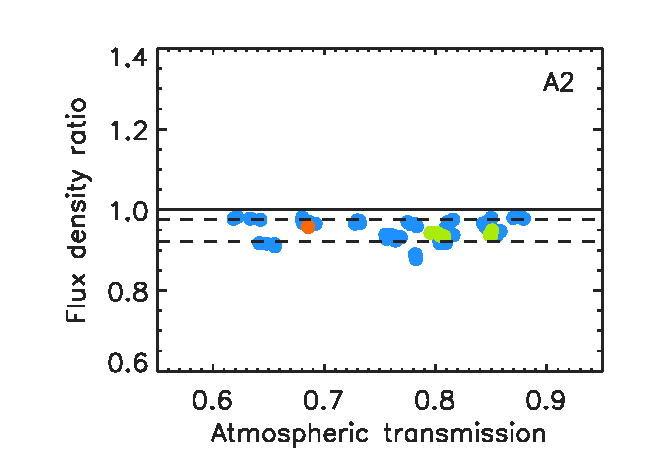
\includegraphics[clip=true, trim={1.8cm, 0.2cm, 0.5cm, 0.7cm},width=0.457\linewidth]{Figures/plot_flux_density_ratio_MWC349_obstau_corrected_skydip_narrow_a2.pdf}
    \begin{overpic}[clip=true, trim={0.9cm, 0.2cm, 0, 0.6cm},width=0.532\linewidth]{Figures/plot_flux_density_ratio_MWC349_obstau_tau225_narrow_1mm.pdf}
      \put(20,60){\footnotesize Taumeter}
    \end{overpic}
    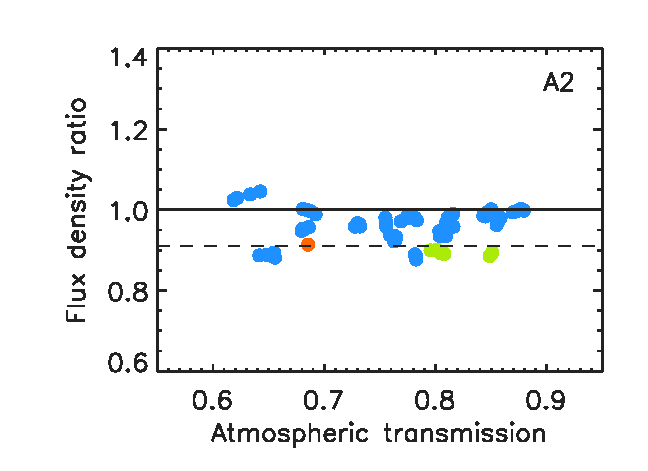
\includegraphics[clip=true, trim={1.8cm, 0.2cm, 0.5cm, 0.7cm},width=0.457\linewidth]{Figures/plot_flux_density_ratio_MWC349_obstau_tau225_narrow_a2.pdf}
    \begin{overpic}[clip=true, trim={0.9cm, 0.2cm, 0, 0.6cm},width=0.532\linewidth]{Figures/plot_flux_density_ratio_MWC349_obstau_skydip_narrow_1mm.pdf}
      \put(20,60){\footnotesize Skydip}
    \end{overpic}
    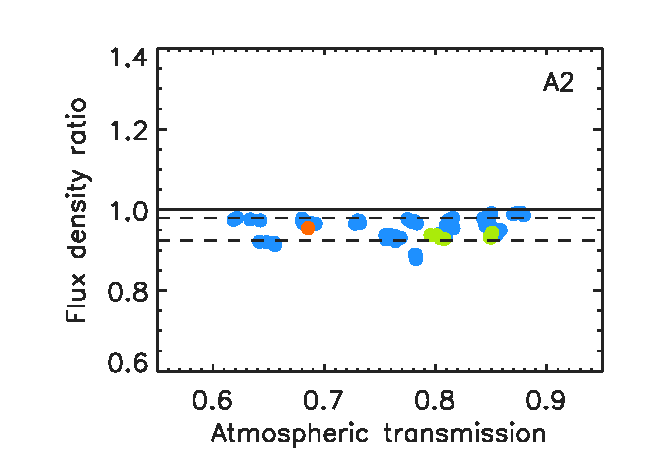
\includegraphics[clip=true, trim={1.8cm, 0.2cm, 0.5cm, 0.7cm},width=0.457\linewidth]{Figures/plot_flux_density_ratio_MWC349_obstau_skydip_narrow_a2.pdf}
    \begin{overpic}[clip=true, trim={0.9cm, 0.2cm, 0, 0.6cm},width=0.532\linewidth]{Figures/plot_flux_density_ratio_MWC349_obstau_corrected_skydip_photocorr_demo_narrow_1mm.pdf}
      \put(20,60){\footnotesize Photocorr Demo}
    \end{overpic}
    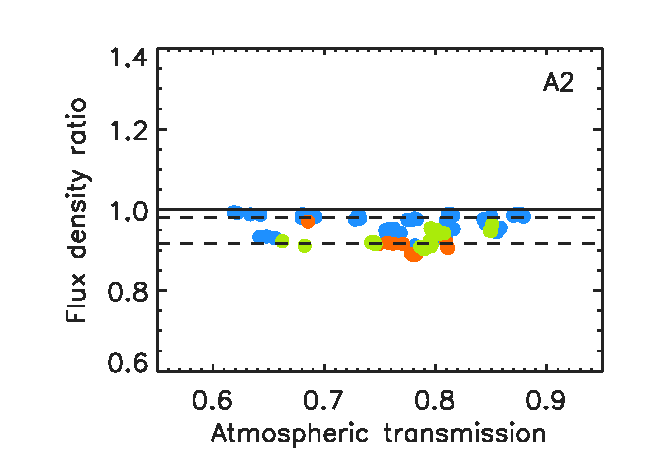
\includegraphics[clip=true, trim={1.8cm, 0.2cm, 0.5cm, 0.7cm},width=0.457\linewidth]{Figures/plot_flux_density_ratio_MWC349_obstau_corrected_skydip_photocorr_demo_narrow_a2.pdf}
    \begin{overpic}[clip=true, trim={0.9cm, 0.4cm, 0, 0.6cm},width=0.532\linewidth]{Figures/plot_flux_density_ratio_MWC349_obstau_corrected_skydip_photocorr_pointing_narrow_1mm.pdf}
      \put(20,60){\footnotesize Photocorr Pointing}
    \end{overpic}
    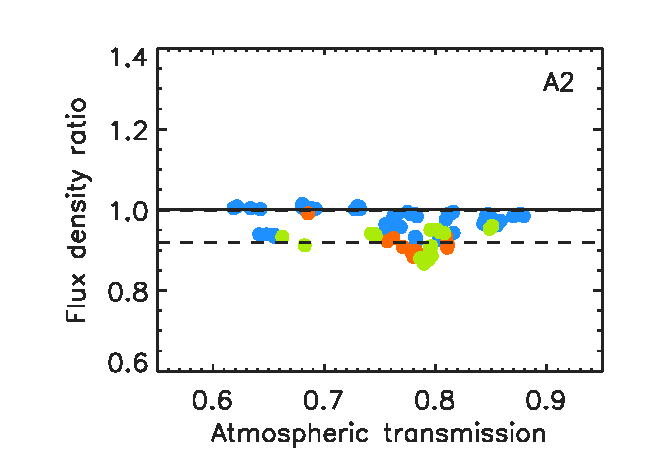
\includegraphics[clip=true, trim={1.8cm, 0.4cm, 0.5cm, 0.7cm},width=0.457\linewidth]{Figures/plot_flux_density_ratio_MWC349_obstau_corrected_skydip_photocorr_pointing_narrow_a2.pdf}
    \vspace{-0.3cm}
    \caption[Calibration bias comparison]{Comparison of the
        calibration bias for five calibration methods using
          observations of MWC349.
       The measured-to-expected flux density ratio is shown as a
      function of the atmospheric transmission for the baseline method
      (first row) as well as for methods using the {\tt taumeter} (second
      row) and {\tt skydip} (third) opacity correction, and for methods
      resorting to the {\tt PC-demo} (fourth) and {\tt PC-point} (fifth)
      photometric correction. Dashed lines
      show the flux density ratio $1 \sigma $ dispersion.}
    \label{fig:mwc349_obstau_others}
  \end{center}
\end{figure}

%
\begin{figure}[!thbp]
  \begin{center}
%    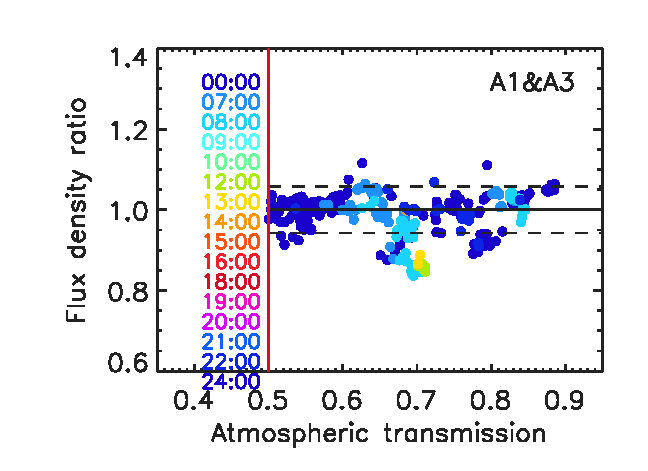
\includegraphics[clip=true, trim={0.9cm, 0.2cm, 0, 0.7cm},width=0.532\linewidth]{Figures/plot_flux_density_ratio_obstau_allbright_obsdate_corrected_skydip_narrow_1mm.pdf}
%    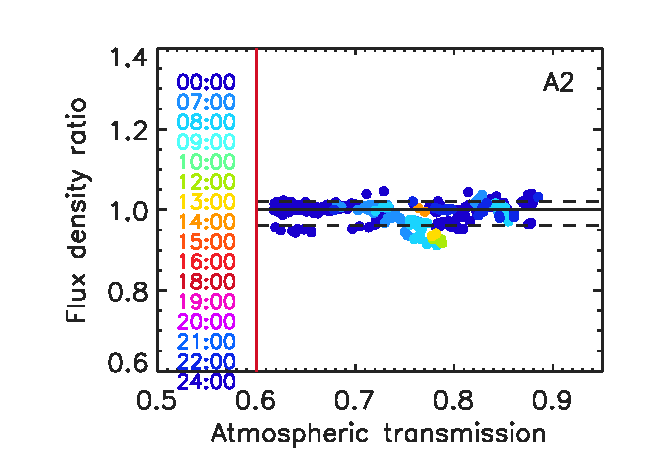
\includegraphics[clip=true, trim={1.8cm, 0.2cm, 0.5cm, 0.7cm},width=0.455\linewidth]{Figures/plot_flux_density_ratio_obstau_allbright_obsdate_corrected_skydip_narrow_a2.pdf}
%    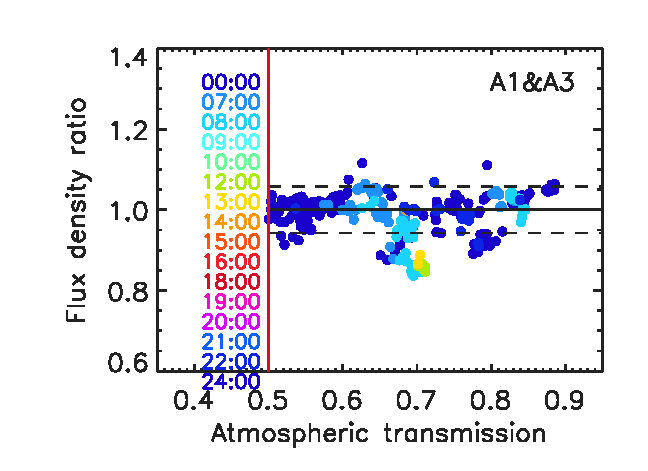
\includegraphics[clip=true, trim={0.9cm, 0.2cm, 0.5cm, 0.7cm},width=0.65\linewidth]{Figures/plot_flux_density_ratio_obstau_allbright_obsdate_corrected_skydip_narrow_1mm.pdf}
%     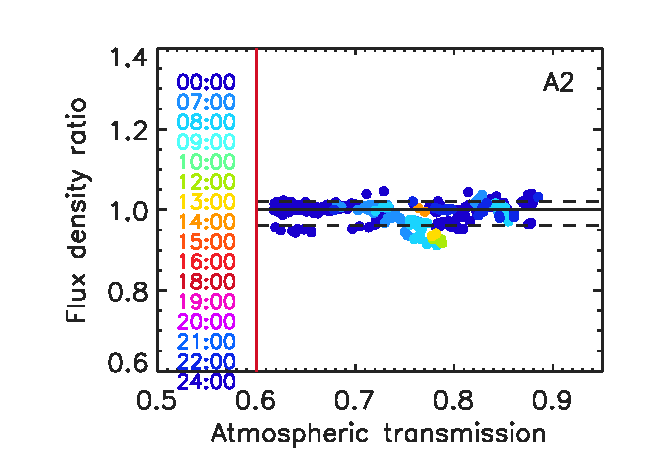
\includegraphics[clip=true, trim={0.9cm, 0.2cm, 0.5cm, 0.7cm},width=0.65\linewidth]{Figures/plot_flux_density_ratio_obstau_allbright_obsdate_corrected_skydip_narrow_a2.pdf}
      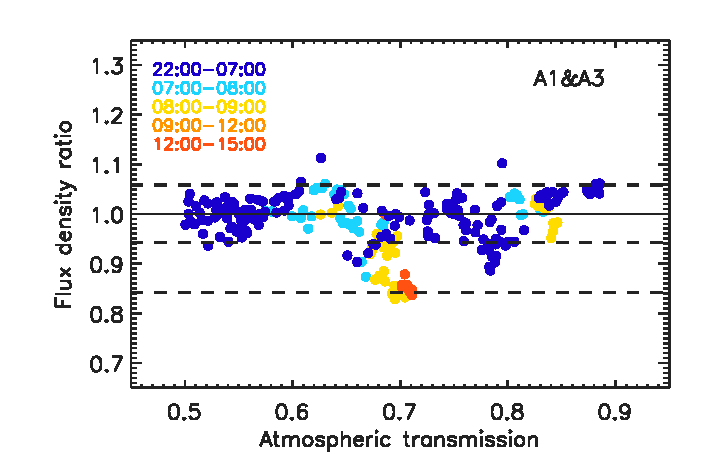
\includegraphics[clip=true, trim={0.9cm, 0, 0.5cm, 0.6cm},width=0.75\linewidth]{Figures/plot_flux_density_ratio_obstau_allbright_obsdate_corrected_skydip_rescaled_1mm.pdf}
     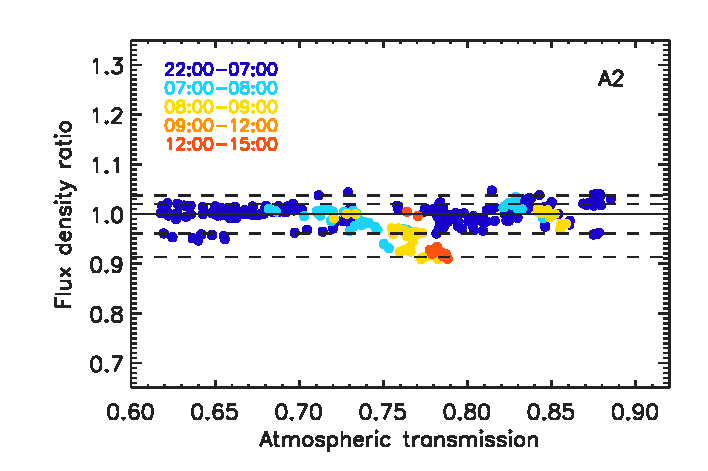
\includegraphics[clip=true, trim={0.9cm, 0, 0.5cm, 0.6cm},width=0.75\linewidth]{Figures/plot_flux_density_ratio_obstau_allbright_obsdate_corrected_skydip_rescaled_a2.pdf} 


    \caption[Baseline calibration rms error estimate]{Baseline
      calibration uncertainties. The
      measured-to-median flux density ratio of bright sources is
      plotted as a function of the atmospheric transmission
      color-coded according to the UT
      observation time of the scans for the combination of A1$\&$A3
      (top pannel)
      and for A2 (bottom pannel).
      The inner dashed lines from either sides of the
      unity-ratio line show the rms errors, {\lp which
      are less than 6\% at $1\,\rm{mm}$ and 3\% at $2\,\rm{mm}$, while
      the outer dashed lines show the $95\%$ confidence level contours.}
      The lowest flux ratio data points correspond to some of the
      scans acquired during daytime between 8:00 UT and 15:00 UT
      hours (yellow and red), while the scans acquired during nightime
      between 22:00 UT and 7:00 UT yield data points (dark blue)
      well distributed within the rms error with a few outliers.}
    \label{fig:allbright_rms_corrected_skydip}
  \end{center}
\end{figure}




%---------------------------------------------------------------------
%	Comparaison
%---------------------------------------------------------------------
\subsection{Comparison with other calibration methods}
\label{se:photometry_others}

% ALL METHOD RESULTS 
\begin{table*}[!htbp]
\begin{center}
\begin{tabular}{clrrrrr}
  \hline\hline
  \noalign{\smallskip}
  \multicolumn{2}{c}{}  &  \multicolumn{5}{c}{Methods} \\\cline{3-7}
  \noalign{\smallskip}
  \multicolumn{2}{c}{Characteristics} &  baseline  & {\small {\tt taumeter}}  & {\small {\tt skydip}}  &  {\small {\tt PC-demo}} & {\small {\tt PC-point}} \\
  \hline
  \noalign{\smallskip}
  %Bias &  $\#$ total    &   109   &   109    &   109    &    109    &  109   \\
  %     &  $\#$ selected &    72   &   72     &    72    &     96    &   95   \\
  %     &  A1            &   0.98  &  1.01    &  0.99    &   0.98    &  1.00  \\
  %     &  A3            &   1.00  &  1.04    &  1.01    &   1.01    &  1.02  \\
  %     &  1mm           &   1.00  &  1.03    &  1.00    &   1.00    &  1.01  \\
  %     &  2mm           &   0.95  &  0.96    &  0.95    &   0.95    &  0.95  \\
  %\hline
  %\multicolumn{7}{|l|}{Using color corrections as of Table A.1} \\
  %\hline
  Bias &  A1            &   0.95   &  0.98    &  0.97    &   0.95    &  0.97  \\
       &  A3            &   1.00   &  1.02    &  1.02    &   0.99    &  1.00  \\
       &  1mm           &   0.98   &  1.01    &  1.00    &   0.97    &  0.99  \\
       &  2mm           &   0.95   &  0.95    &  0.95    &   0.95    &  0.95  \\
  \hline
  \noalign{\smallskip}
  Rms  &  $\#$ total    &   487    &    487   &    487    &    396    &  396 \\
  $[\%]$ &  $\#$ selected &   264    &    264   &    264    &    291    &  283 \\
       &  A1            &   5.5    &    7.5   &    7.3    &    4.0    &  4.9 \\
       &  A3            &   6.0    &    8.1   &    7.1    &    4.1    &  5.2 \\
       &  1mm           &   5.7    &    7.9   &    7.1    &    3.8    &  4.9 \\
       &  2mm           &   3.0    &    3.8   &    3.0    &    2.2    &  2.4 \\
\hline
\end{tabular}
\caption[Comparison of calibration results using five
  methods]{Comparison of results using five calibration methods.}
\label{tab:Calibration_results_all}
\end{center}
\end{table*}

In this section, the \emph{baseline} calibration results are compared to
results drawn either using other calibration methods obtained from different
opacity corrections ({\tt taumeter} and {\tt skydip} as
discussed in Sect.~\ref{se:baseline_calibration_opacity}), or
including a photometric correction ({\tt PC-demo} and {\tt PC-point},
as described in Sect.~\ref{se:photometric_correction}). For robustness test, we
evaluate and compare the photometry quality critera of
Sect.~\ref{se:photometry_criteria} for the five calibration methods.


\subsubsection{Calibration bias}
\label{se:calibration_bias_all}

We present the calibration bias as a function of the atmospheric
transmission for the five calibration methods in
Fig.~\ref{fig:mwc349_obstau_others} and report the results in the row
labelled 'Bias' of Table~\ref{tab:Calibration_results_all}.

At $1\,\rm{mm}$, all methods lead to flux density estimates in
agreement with expectations within the rms dispersion. However,
{\tt taumeter} flux ratios have more dispersion than
the \emph{baseline} flux ratios whereas {\tt skydip} shows some
dependency on the atmospheric
transmission, with a 10 to $15\%$ excess of the flux density with
respect to expectations at high transmission. Indeed this residual
systematic effect has motivated the development of the {\tt corrected
  skydip} method, as discussed in
Sect.~\ref{se:corrected-skydip}. These features, which are
already noticeable from Fig.~\ref{fig:mwc349_obstau_others}, will be
confirmed and further discussed later using more observation scans. On
the other hand, the calibration methods based on photometric
correction (Sect.~\ref{se:photometric_correction}) yield an
unbiased photometry (calibration bias in agreement with unity
within the rms error) while allowing the use of $30\%$ more
scans. These results are encouraging for the exploitation of scans
acquired during the observing periods
impacted by the \afternoon\ beam variation effect
(Sect.~\ref{se:beam_variation}).

At $2\,\rm{mm}$, all methods result in a similar calibration bias
of $0.95 \pm 0.05$, which corresponds to a low-significance $5\%$
lack of flux density toward MWC349.
%We also obtained the same calibration
%biases for each observation campaign (see
%Table~\ref{tab:baseline-photometry}).
To summarize, the calibration bias at $2\, \rm{mm}$ is stable against
i) a large range of atmospheric conditions, ii) the observation campaign, iii) the
opacity correction method, iv) the method to treat the
temperature-induced beam variation effect.
%An explanation for the
%$5\%$ lack of flux density toward
%MWC349 is probably to be seeked on the side of the flux density
%expectations for this source.
This $5\%$ lack of flux density is thus probably due to
uncertainties on the flux density expectations for this source.
They come in two flavours.
{\lp Firstly the uncertainties on the flux expectation, as reported in
Appendix~\ref{se:ref_flux_secondaries}, consist in the propagation of
the errors on the fitted SED from PdBI and VLA observations. Systematic
uncertainties that may also impact the SED are not included.}  
%the accuracy of the SED fitted from PdBI and VLA observations
%(see Sect.~\ref{se:ref_flux_secondaries})
%depends on these instruments absolute flux density calibration, which
%is at least greater than the $5\%$ primary calibrator model accuracy,
Secondly, the NIKA2 flux density extrapolation from
interferometer data may be not straightforward for MWC349. {\lp In
particular, NIKA2 flux extrapolation ignores the contamination by
strong masers in the radio recombination lines~\citep{masingRRL},
while strong maser emission lines are masked in PdBI observations to
measure the continuum. In addition, the resulting continuum shows
indications of variability.}


\subsubsection{Calibration uncertainties}

The calibration uncertainties for the five methods evaluated using
flux-selected source scans are gathered in the subpanel labelled 'Rms'
of Table~\ref{tab:Calibration_results_all}.

Compared to the baseline method, the {\tt taumeter} method leads to 
statistical uncertainty increased of about $40$ and $30\%$ at 1 and
$2\,\rm{mm}$. The {\tt skydip} method shows lower dispersion but a
mild correlation with the atmospheric transmission, as
discussed in Sect.~\ref{se:calibration_bias_all}.

In addition, we have checked the flux density ratios for the bunch of
scans with an atmospheric transmission of about 0.7, which were
discussed in Sect.~\ref{se:photometry_baseline}, by comparing
calibration methods with or without photometry correction. Whereas the
flux density ratios are low for the scans observed within 12:00 and
15:00 UT in the three first
methods, they are within the 68\% C.L. interval when using a photometric
correction. This further validates the hypothesis that the low flux
density of these scans is due to \afternoon\ beam effect, as assumed in
Sect.~\ref{se:photometry_baseline}. This also constitutes an example
of the calibration improvement obtained from resorting to a
photometric correction.

Moreover, results based on the {\tt PC-demo} method show that rms calibration
uncertainties as low as $3.8$ and $2.2\%$
at 1 and $2\,\rm{mm}$ are within the reach of NIKA2 {\lp without any
selection based on the observation time.}
%without rejecting any observations.
However, we recall this method relies on 
accurate beam estimates. Using {\tt PC-point}, which is the
practical case, still improves the calibration uncertainties
w.r.t. the baseline results but by a factor of about $20\%$ in both
bands. However, the differences between
the flux density ratios from {\tt PC-demo} and {\tt PC-point}, which are
seen e.g. from the 'photocorr demo' and 'photocorr pointing' of
Fig.~\ref{fig:mwc349_obstau_others}, are likely
to be due to the photometry correction noise
when monitoring the beam from pointing scans. We conclude that more
control on the beam monitoring is needed before routinely using a calibration
based on photometry correction. By contast, the baseline method
combines good performance with robustness.


\paragraph{Summary} Among the methods that rely on the UT hour-based
scan selection to mitigate the effect of beam size variations, the
baseline method shows the best performance in terms of calibration
bias and uncertainties. The methods that rely on a photometric correction
lead to good calibration results, and thus represent a promising lead
to further improve the calibration uncertainties. However, their
robustness depends on the accuracy of the beam monitoring. {\lp The
proposed beam monitoring based on {\tt pointing} scans induces some
extra dispersion of the flux densities. A more accurate beam monitoring is
feasable but requires using dedicated observation scans.} 
Using the baseline method, the measured flux density of
MWC349 is in agreement with expectations within $5\%$ for both
wavelengths. Moreover, we find calibration uncertainties of $5.7\%$ at
$1\,\rm{mm}$ and $3\%$ at $2\,\rm{mm}$ using a series of 264 scans of
sources of flux density above $1\, \rm{Jy}/\rm{beam}$. These results
demonstrate the excellent accuracy and stability of the NIKA2
photometric capabilities.







NIKA2 photometric capabilities after the calibration presented in
Sect.~\ref{se:calibration}, are assessed in this section. Firstly,
we use observation of secondary calibrators (planetary nebulae NGC7027, CRL2688, and
MWC349A) to test the consistency of the flux density estimates with
expectations. The flux density expectations
in NIKA2 bands for these calibrators are given in
Appendix~\ref{se:ref_flux_secondaries}. Then,
we verify the stability of the photometry with
respect to the atmospheric conditions using a large amount of
observations toward a large variety of sources. 

The quality criteria used to assess the photometric
capabilities and calibration results are defined in
Sect.~\ref{se:photometry_criteria}.
In Sect.~\ref{se:photometry_baseline}, these criteria are evaluated
for the baseline calibration, and in Sect.~\ref{se:photometry_others},
we compare these results with other calibration method results. 


%---------------------------------------------------------------------
%	Criteria
%---------------------------------------------------------------------
\subsection{Calibration accuracy and uncertainty assessment}
\label{se:photometry_criteria}

We assess the photometric performance by evaluating two
quality criteria: first, the calibration bias checks the accuracy of
the absolute calibration and then the calibration relative
uncertainties test the stability of the flux densities. \\

\noindent \emph{Calibration bias} We define the calibration bias
$b_{\nu}$, where $\nu$ stands for Array 1, 2, 3 and the
$1\,\rm{mm}$ array combination, as
the ratio between the measured flux density $\hat{S}_{\nu}$ using the
%fixed-width Gaussian beam
reference photometry
(Sect.~\ref{se:photometric_system}) and the flux density
expectations $S_{\rm{s}}(\nu_0)$ as given in
Appendix~\ref{se:ref_flux_secondaries}. From a series of
secondary calibrator scans, we evaluate the average calibration bias
$b_{\nu}$, which by construction, should be equal to
unity within uncertainties.
%the precision with which the expected flux densities are known.
Moreover, we check the stability of the calibration bias against
the observed opacities as a robustness test of the
opacity derivation method. Likewise, we verify that the photometry is
insensitive to optical variations by checking the stability of the
calibration bias against the measured beam size.\\

\noindent \emph{Calibration uncertainties} We evaluate the standard
deviation of bright source measured-to-median flux density ratio
$\sigma_{\nu}$ per array or array combination $\nu$. {\lp Since the flux
density ratios are not Gaussian distributed, we
evaluate the 68 and 95\% confidence level (C.L.) contours using the
measured distributions in order to further characterise the
uncertainties. We check that the rms
errors are larger than the 68\% C.L. contours and thus provide
conservative $1\sigma$-like errors.}    

As the flux density of most of the considered sources is unknown a priori, we
compare the flux density estimate in a single observation scan to the
average flux density throughout an observation campaign. This method
requires the selection of sources that are bright enough to be detected with a high
signal-to-noise ratio with a single repetition of an usual
$8'\times 5'$ OTF raster scan. Namely, we perform a source
selection by thresholding the flux estimate to $800\,\rm{mJy}$ at
$1\,\rm{mm}$ and $400\,\rm{mJy}$ at $2\,\rm{mm}$. Moreover, we consider
only the sources for which a minimum of $10$ scans are available after
selection to ensure a precise average flux density
estimation. Finally, the selected source scans must meet the \emph{baseline}
scan selection criteria given in Sect.~\ref{se:data_selection}.

{\lp As the rms of the flux density ratio is estimated on a scan set
that is representative of the observing conditions encountered at
the \trentemetre\ telescope, this is an estimate of the
calibration uncertainties that encloses errors of
optical, atmospheric, instrumental noise and data processing
origins. This includes the errors sourced by the \afternoon\ beam 
variations, the effect of the elevation, the uncertainties of the
atmospheric opacity correction using either the {\tt skydip} or
the {\tt taumeter} method and the atmospheric and instrumental noise
residuals after the data reduction (Sect.~\ref{se:dataproc}).

To obtain an estimate of the total absolute
calibration uncertainties, the rms errors must be added in quadrature
with systematic uncertainties that do not depend on the observing
conditions. The main source of systematic error is the model uncertainty
on the primary calibrator flux density expectations. In the case of
Uranus, \citet{Morenothesis} and \citet{Bendo2013} report model
uncertainties of about $5\%$ at both wavelenghts.

When using the \emph{baseline}
calibration method, which resorts to the {\tt corrected skydip} method
for the atmospheric opacity correction (see
Sect.~\ref{se:corrected-skydip}), the uncertainties on the
correcting factor $a_\nu^{\rm{skydip}}$, as defined in
Eq.~\ref{eq:corrected_skydip}, must be propagated to the flux
uncertainties. These uncertainties, which are referred to as the
{\tt corrected skydip} uncertainties, depend on the line-of-sight atmospheric
opacity $\taunu x$. Precisely, because the {\tt corrected skydip}
opacity correction is consistently used for both the primary
calibrator and the target source flux measurement, the {\tt corrected skydip}
uncertainties depends on the difference between the average
line-of-sight opacity of the primary calibrator scans and the
line-of-sight opacity of the source scan.   
We evaluate the {\tt corrected skydip} uncertainties for two
different $\taunu x$ values. First for the reference IRAM \trentemetre\
winter observing conditions, as defined as $2\,\rm{mm}$ of pwv and an
elevation of $60^{\rm{o}}$, the {\tt corrected skydip} uncertainties are of
0.6\% at $1\,\rm{mm}$ and 0.3\% at $2\,\rm{mm}$. Secondly in the worst
observing conditions allowed by the \emph{baseline} scan selection,
which are $\taunu x$ of 0.7 at $1\,\rm{mm}$ and of 0.5 at
$2\,\rm{mm}$, we find {\tt corrected skydip} uncertainties of 2\% and
$1.5\%$ at 1 and $2\,\rm{mm}$, respectively. These constitute
conservative upper limits on the {\tt corrected skydip}
uncertainties.

The uncertainties on NIKA2 bandpass measurements (see
Sect.~\ref{se:instru_bandpass}) propagate into
uncertainties on the flux densities after the color correction using
Eq.~\ref{eq:color_correction}. These
uncertainties depend on the source SED but are neglectible in most of
the cases. In particular, for MWC349, we find uncertainties below 0.1\% at
both wavelengths.}





%---------------------------------------------------------------------
%	Baseline results
%---------------------------------------------------------------------
\subsection{Baseline calibration photometry results}
\label{se:photometry_baseline}

We measure the calibration bias and statistical uncertainties, as defined
in the previous section (Sect.~\ref{se:photometry_criteria}) using the
\emph{baseline} calibration method (Sect.~\ref{se:baseline_calibration}).

%  BASELINE RESULTS
%%%%%%%%%%%%%%%%%%%%%%%%%%%%%%%%%%%%%%%%%%%%%%%%%%%%%%%%%%%%%%%%%%
\begin{table}[!thbp]
  \begin{center}
    \caption[Baseline calibration results]{Baseline calibration results:
  photometry accuracy and uncertainties. The first subpanel labelled 'Bias' gives the
  calibration bias $b_{\nu}$ and the second subpanel labelled 'Rms' the calibration
  rms error $\sigma_{\nu}$, as defined in
  Sect.~\ref{se:photometry_criteria},
  using observations during N2R9, N2R12, N2R14 and the combination of
  the three campaigns. {\lp In each subpanel, the first row indicates the
    number of acquired scans, while the second row gives the
    number of selected scans using the \emph{baseline} scan selection.}}
\label{tab:baseline-photometry}
\begin{tabular}{clrrrr}
  \hline\hline
  \noalign{\smallskip}
 % \multicolumn{2}{c}{}  &  \multicolumn{4}{|c}{Datasets}  \\\cline{3-6}
  \multicolumn{2}{c}{Characteristics} &  N2R9  & N2R12   &  N2R14 & Combined \\
  \noalign{\smallskip}
  \hline
  \noalign{\smallskip}
%  Bias &  $\#$ total    &  68    &  14     &   27     &    109    \\
%       &  $\#$ selected &  64    &   1     &   7      &     72    \\
%       &  A1            &  0.99  &  1.06   &   0.98   &   0.98    \\
%       &  A3            &  1.01  &  1.08   &   1.04   &   1.00    \\
%       &  1mm           &  1.00  &  1.07   &   1.01   &   0.99    \\
%       &  2mm           &  0.95  &  0.96   &   0.94   &   0.95    \\
%  \hline
%  \multicolumn{6}{|l|}{using color corrections as of Table A.1}  \\
%  \hline
  Bias &  $\#$ total    &  68    &  14     &   27     &    109    \\
       &  $\#$ selected &  64    &   1     &   7      &     72    \\
       &  A1            &  0.95  &  1.03   &   0.94   &   0.95    \\
       &  A3            &  0.99  &  1.07   &   1.00   &   1.00    \\
       &  1mm           &  0.97  &  1.05   &   0.97   &   0.98    \\
       &  2mm           &  0.95  &  0.95   &   0.93   &   0.95    \\
  \hline
  \noalign{\smallskip}
  Rms  &  $\#$ total    &  303   &  72     &   112    &    487   \\
  $[\%]$ &  $\#$ selected &  219   &  33     &    12    &    264   \\
       &  A1            &  5.7   &  4.6    &   2.9    &    5.5   \\
       &  A3            &  6.2   &  5.7    &   2.4    &    6.0   \\
       &  1mm           &  5.9   &  5.0    &   2.5    &    5.7   \\
       &  2mm           &  3.2   &  2.1    &   1.1    &    3.0   \\  
\hline
\end{tabular}
\end{center}
\end{table}

The calibration bias is evaluated using a
series of scans of MWC349 acquired during the
%N2R9, N2R12 and N2R14
 reference observation campaigns. Namely, we use the 72 scans that met
 the \emph{baseline} selection
 criteria (see Sect.~\ref{se:data_selection}) over the 109 available
scans for MWC349. The first row of
Fig.~\ref{fig:mwc349_obstau_others}, labelled 'baseline', shows the
calibration bias $b_{\nu}$ for the combination of the $1\,\rm{mm}$ arrays and
Array 2 as a function of the atmospheric transmission %, which is
%evaluated with the zenith opacity $\taunu$ and the airmass $x$ as
$\exp \left( - \taunu \, x \right)$. No significant dependency of the
calibration bias on the atmospheric transmission is observed. 

Table~\ref{tab:baseline-photometry} gathers the calibration bias
estimates for the three observation campaigns and for all the scans.
In the $1\,\rm{mm}$ band, we find
$b_\nu$ in agreement with unity within the statistical dispersion for
the three campaigns,
whereas a $5\%$ lack of flux with respect to expectations is observed
at $2\,\rm{mm}$, consistently for the three campaigns. This bias has a
low significance with respect to the absolute calibration precision of
NIKA2 (see Sect.~\ref{se:photometry_criteria}).
%{\lp Furthermore, the flux density expectations have also
%uncertainties.}
%and PdBI, which depend on the precicision with which the
%primary calibrator flux densities are known. For Uranus, the model
%uncertainties are of about $5\%$, as reported
%in~\citet{Morenothesis,Bendo2013}. 
This will be further investigated by using other calibration methods
in Sect.~\ref{se:photometry_others}.


%The baseline calibration relative uncertaintes, as defined in
%Sect.~\ref{se:photometry_criteria}, are evaluated using bright
%sources. From a total of 487 scans
%flux-selected sources acquired during N2R9, N2R12 and N2R14, 264 met
%the baseline selection criteria and are used for testing stability.
Figure~\ref{fig:allbright_rms_corrected_skydip} shows the
measured-to-median flux densities evaluated from bright source scans
for the combination of Array $1\&3$ and Array 2 as a function of the
atmospheric transmission and color-coded as a function of the
observation time. From a total of 487 scans towards
flux-selected sources, acquired during N2R9, N2R12 and N2R14, 264 met
the baseline selection criteria and are included in
Fig.~\ref{fig:allbright_rms_corrected_skydip} for testing the
calibration stability. The statistical calibration uncertainties are
estimated using the standard deviation of the flux density ratios for
the three campaigns. Results are gathered in
Table~\ref{tab:baseline-photometry}.
Combining all the scans, we find uncertainties of $5.5\%$ for A1,
$6.0\%$ for A3, $5.7\%$ for the $1\,\rm{mm}$ band and $3.0\%$ for A2.
%%%%%%% 95% %%%%%%%%%%%%%%%%%%%%%%%%
{\lp Using the flux ratio distributions, we construct the 68 and 95\%
C.L. intervals. The 68\% C.L. intervals are $-6.4\%$ and $+3.4\%$ at
$1\,\rm{mm}$ and $-3.8\%$ and $+1.5\%$ at $2\, \rm{mm}$. Hence in average
the 68\% C. L. errors are of $4.9\%$ and $2.7\%$ at 1 and $2\, \rm{mm}$,
respectively. We conclude that the rms errors are conservative
estimates of the 68\% C. L. errors at both wavelengths. The 95\%
C.L. contours are $-15.8\%$ and $+5.9\%$ at $1\,\rm{mm}$ and $-8.6\%$ and
$+3.8\%$ at $2\, \rm{mm}$.
The rms errors and the 95\%
C.L. interval are shown in
Fig.~\ref{fig:allbright_rms_corrected_skydip} with the inner and
outter dashed lines, respectively.} 


The flux density ratio is constant within the rms errors along the
wide range of tested atmospheric transmission, ranging from 0.5 to 0.9
at $1\,\rm{mm}$.
However, some scans at atmospheric transmissions of about 0.7 at
$1\,\rm{mm}$ show a mild lack of flux density with respect to the
median within the 95\% C. L. contours. The scans
affected by the lack of flux have all been observed
either between 12:00 and 14:00 UT or between 8:00 and 9:00 UT,
that are close to the threshold of the observation time cuts of
the \emph{baseline} scan selection (see
Sect.~\ref{se:data_selection}). These scans are likely
to be affected by the \afternoon\ beam broadening or by the
sunrise focus drift, respectively. Furthermore, we find that restricting the
used observation time to the 10 more stable hours (from 22:00 to
08:00 UT) would result in rms calibration uncertainties of
$3.6\%$ at $1\,\rm{mm}$ and $1.2\%$ at $2\,\rm{mm}$, which constitute an
improvement of about $60\%$ at $1\,\rm{mm}$ and $40\%$ at $2\,\rm{mm}$
of the rms errors.  
The \emph{baseline} scan selection, which i)
retains 16 hours of observation time
a day and ii) %results in calibration uncertainties that meet the
%requirement for a millimetric ground-based instrument,
{\lp results in state-of-the-art statistical calibration
uncertainties,} constitutes an advantageous tradeoff.

%%%%%%%%%%%%%%%%%%%%%%%%%%%%%%%%%%%%%%%%%%%%%%%%%%%%%%%%%%%%%%%%%%%%%%%%%%%%%%%%%%%%%%%%%%%%%
%                              bias
\begin{figure}[!thbp]
  \begin{center}
    \begin{overpic}[clip=true, trim={0.9cm, 0.2cm, 0, 0.6cm},width=0.532\linewidth]{Figures/plot_flux_density_ratio_MWC349_obstau_corrected_skydip_narrow_1mm.pdf}
      \put(20,60){\footnotesize Baseline}
    \end{overpic}
    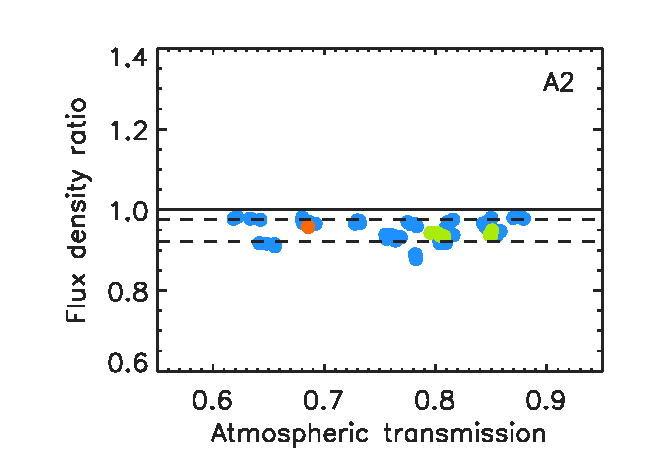
\includegraphics[clip=true, trim={1.8cm, 0.2cm, 0.5cm, 0.7cm},width=0.457\linewidth]{Figures/plot_flux_density_ratio_MWC349_obstau_corrected_skydip_narrow_a2.pdf}
    \begin{overpic}[clip=true, trim={0.9cm, 0.2cm, 0, 0.6cm},width=0.532\linewidth]{Figures/plot_flux_density_ratio_MWC349_obstau_tau225_narrow_1mm.pdf}
      \put(20,60){\footnotesize Taumeter}
    \end{overpic}
    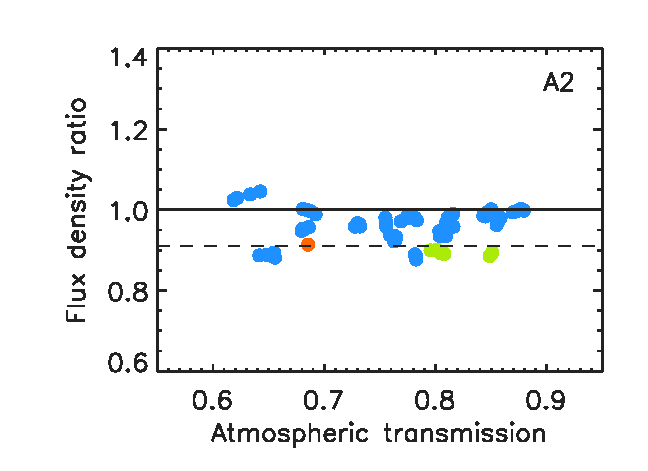
\includegraphics[clip=true, trim={1.8cm, 0.2cm, 0.5cm, 0.7cm},width=0.457\linewidth]{Figures/plot_flux_density_ratio_MWC349_obstau_tau225_narrow_a2.pdf}
    \begin{overpic}[clip=true, trim={0.9cm, 0.2cm, 0, 0.6cm},width=0.532\linewidth]{Figures/plot_flux_density_ratio_MWC349_obstau_skydip_narrow_1mm.pdf}
      \put(20,60){\footnotesize Skydip}
    \end{overpic}
    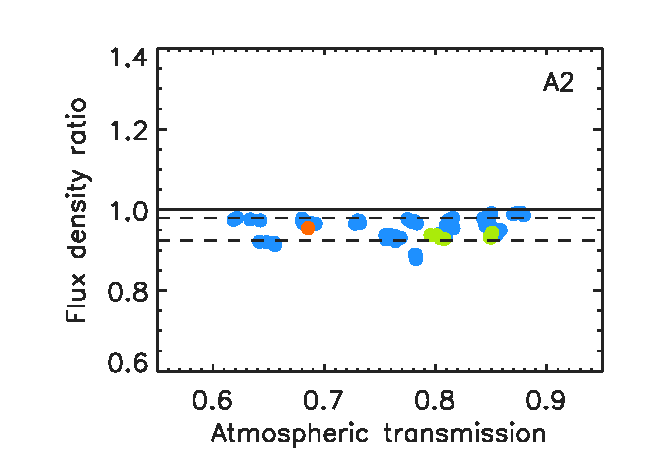
\includegraphics[clip=true, trim={1.8cm, 0.2cm, 0.5cm, 0.7cm},width=0.457\linewidth]{Figures/plot_flux_density_ratio_MWC349_obstau_skydip_narrow_a2.pdf}
    \begin{overpic}[clip=true, trim={0.9cm, 0.2cm, 0, 0.6cm},width=0.532\linewidth]{Figures/plot_flux_density_ratio_MWC349_obstau_corrected_skydip_photocorr_demo_narrow_1mm.pdf}
      \put(20,60){\footnotesize Photocorr Demo}
    \end{overpic}
    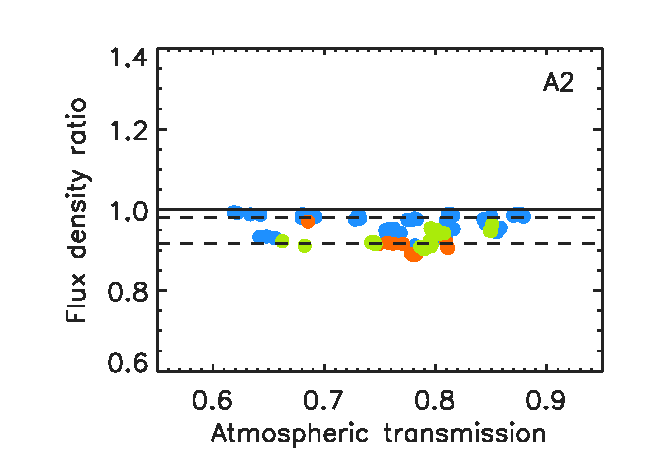
\includegraphics[clip=true, trim={1.8cm, 0.2cm, 0.5cm, 0.7cm},width=0.457\linewidth]{Figures/plot_flux_density_ratio_MWC349_obstau_corrected_skydip_photocorr_demo_narrow_a2.pdf}
    \begin{overpic}[clip=true, trim={0.9cm, 0.4cm, 0, 0.6cm},width=0.532\linewidth]{Figures/plot_flux_density_ratio_MWC349_obstau_corrected_skydip_photocorr_pointing_narrow_1mm.pdf}
      \put(20,60){\footnotesize Photocorr Pointing}
    \end{overpic}
    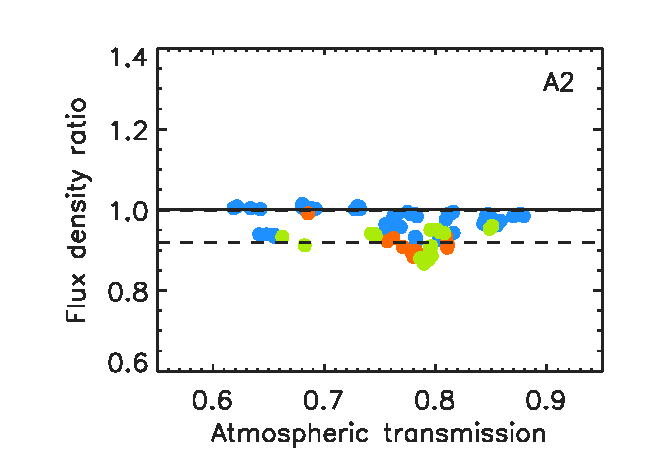
\includegraphics[clip=true, trim={1.8cm, 0.4cm, 0.5cm, 0.7cm},width=0.457\linewidth]{Figures/plot_flux_density_ratio_MWC349_obstau_corrected_skydip_photocorr_pointing_narrow_a2.pdf}
    \vspace{-0.3cm}
    \caption[Calibration bias comparison]{Comparison of the
        calibration bias for five calibration methods using
          observations of MWC349.
       The measured-to-expected flux density ratio is shown as a
      function of the atmospheric transmission for the baseline method
      (first row) as well as for methods using the {\tt taumeter} (second
      row) and {\tt skydip} (third) opacity correction, and for methods
      resorting to the {\tt PC-demo} (fourth) and {\tt PC-point} (fifth)
      photometric correction. Dashed lines
      show the flux density ratio $1 \sigma $ dispersion.}
    \label{fig:mwc349_obstau_others}
  \end{center}
\end{figure}

%
\begin{figure}[!thbp]
  \begin{center}
%    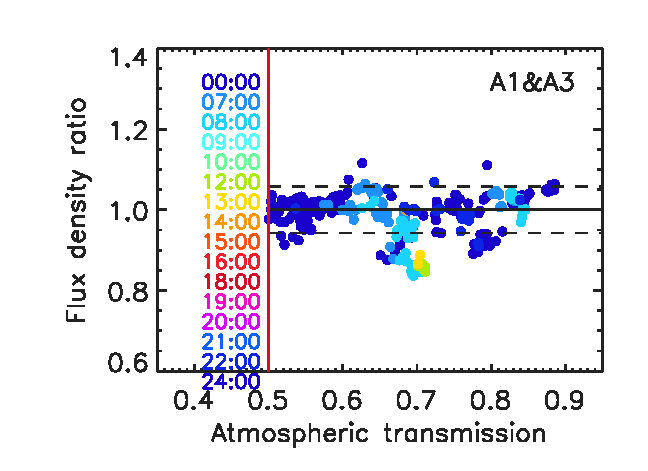
\includegraphics[clip=true, trim={0.9cm, 0.2cm, 0, 0.7cm},width=0.532\linewidth]{Figures/plot_flux_density_ratio_obstau_allbright_obsdate_corrected_skydip_narrow_1mm.pdf}
%    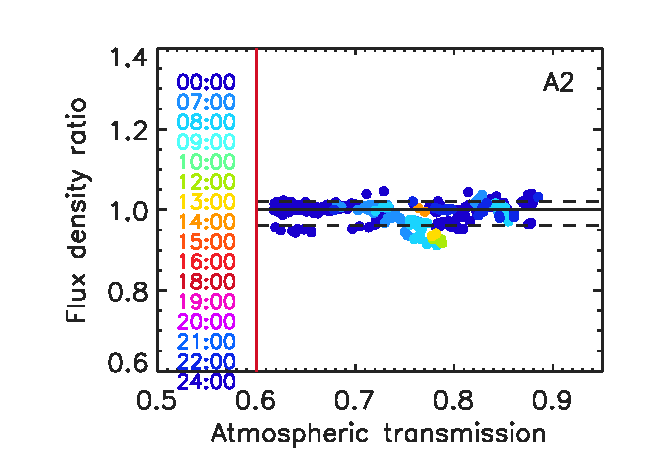
\includegraphics[clip=true, trim={1.8cm, 0.2cm, 0.5cm, 0.7cm},width=0.455\linewidth]{Figures/plot_flux_density_ratio_obstau_allbright_obsdate_corrected_skydip_narrow_a2.pdf}
%    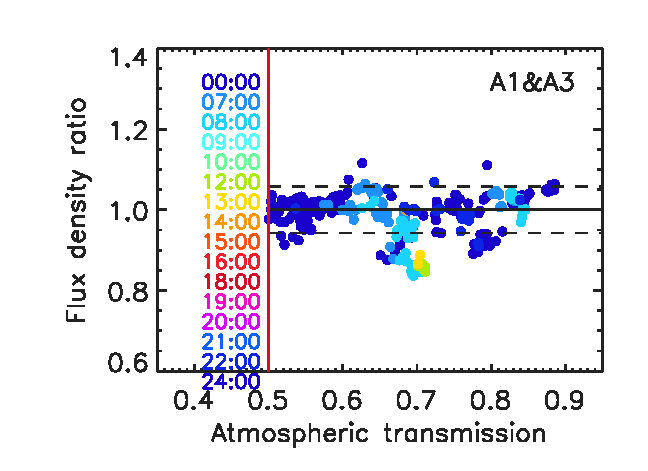
\includegraphics[clip=true, trim={0.9cm, 0.2cm, 0.5cm, 0.7cm},width=0.65\linewidth]{Figures/plot_flux_density_ratio_obstau_allbright_obsdate_corrected_skydip_narrow_1mm.pdf}
%     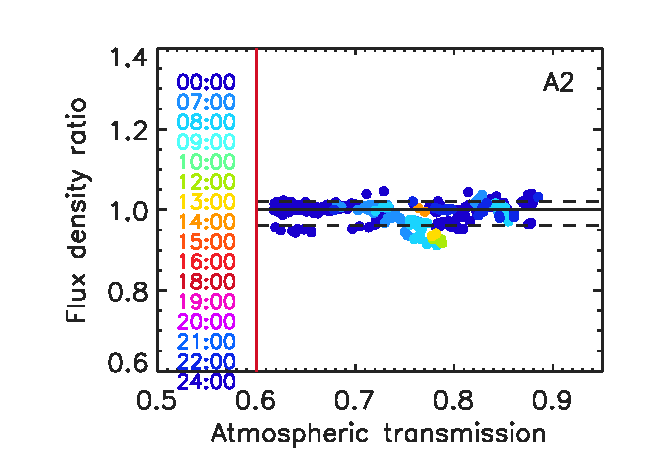
\includegraphics[clip=true, trim={0.9cm, 0.2cm, 0.5cm, 0.7cm},width=0.65\linewidth]{Figures/plot_flux_density_ratio_obstau_allbright_obsdate_corrected_skydip_narrow_a2.pdf}
      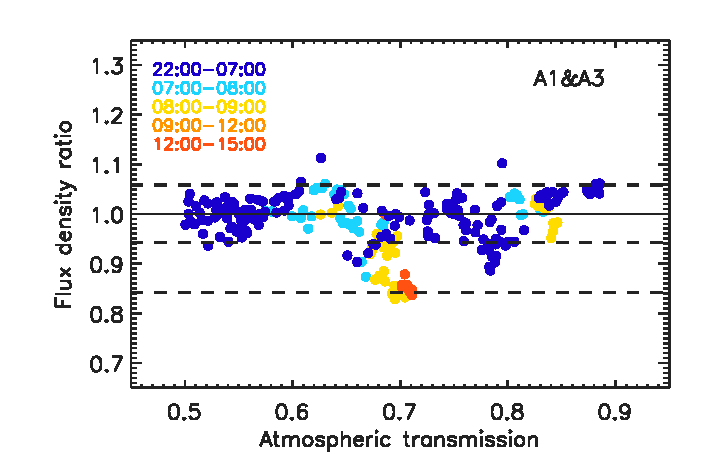
\includegraphics[clip=true, trim={0.9cm, 0, 0.5cm, 0.6cm},width=0.75\linewidth]{Figures/plot_flux_density_ratio_obstau_allbright_obsdate_corrected_skydip_rescaled_1mm.pdf}
     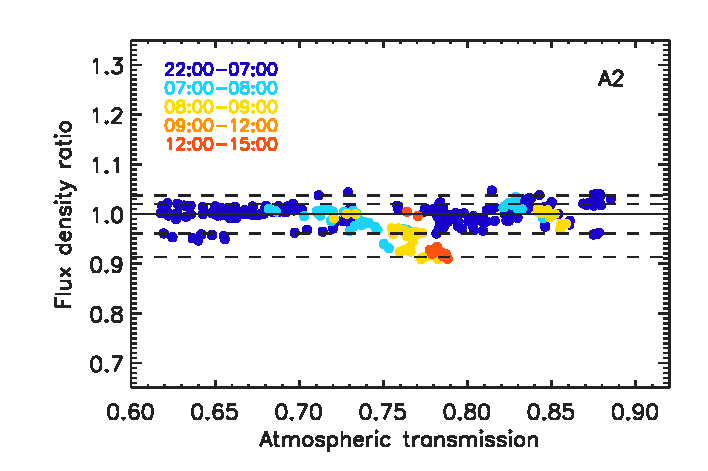
\includegraphics[clip=true, trim={0.9cm, 0, 0.5cm, 0.6cm},width=0.75\linewidth]{Figures/plot_flux_density_ratio_obstau_allbright_obsdate_corrected_skydip_rescaled_a2.pdf} 


    \caption[Baseline calibration rms error estimate]{Baseline
      calibration uncertainties. The
      measured-to-median flux density ratio of bright sources is
      plotted as a function of the atmospheric transmission
      color-coded according to the UT
      observation time of the scans for the combination of A1$\&$A3
      (top pannel)
      and for A2 (bottom pannel).
      The inner dashed lines from either sides of the
      unity-ratio line show the rms errors, {\lp which
      are less than 6\% at $1\,\rm{mm}$ and 3\% at $2\,\rm{mm}$, while
      the outer dashed lines show the $95\%$ confidence level contours.}
      The lowest flux ratio data points correspond to some of the
      scans acquired during daytime between 8:00 UT and 15:00 UT
      hours (yellow and red), while the scans acquired during nightime
      between 22:00 UT and 7:00 UT yield data points (dark blue)
      well distributed within the rms error with a few outliers.}
    \label{fig:allbright_rms_corrected_skydip}
  \end{center}
\end{figure}




%---------------------------------------------------------------------
%	Comparaison
%---------------------------------------------------------------------
\subsection{Comparison with other calibration methods}
\label{se:photometry_others}

% ALL METHOD RESULTS 
\begin{table*}[!htbp]
\begin{center}
\begin{tabular}{clrrrrr}
  \hline\hline
  \noalign{\smallskip}
  \multicolumn{2}{c}{}  &  \multicolumn{5}{c}{Methods} \\\cline{3-7}
  \noalign{\smallskip}
  \multicolumn{2}{c}{Characteristics} &  baseline  & {\small {\tt taumeter}}  & {\small {\tt skydip}}  &  {\small {\tt PC-demo}} & {\small {\tt PC-point}} \\
  \hline
  \noalign{\smallskip}
  %Bias &  $\#$ total    &   109   &   109    &   109    &    109    &  109   \\
  %     &  $\#$ selected &    72   &   72     &    72    &     96    &   95   \\
  %     &  A1            &   0.98  &  1.01    &  0.99    &   0.98    &  1.00  \\
  %     &  A3            &   1.00  &  1.04    &  1.01    &   1.01    &  1.02  \\
  %     &  1mm           &   1.00  &  1.03    &  1.00    &   1.00    &  1.01  \\
  %     &  2mm           &   0.95  &  0.96    &  0.95    &   0.95    &  0.95  \\
  %\hline
  %\multicolumn{7}{|l|}{Using color corrections as of Table A.1} \\
  %\hline
  Bias &  A1            &   0.95   &  0.98    &  0.97    &   0.95    &  0.97  \\
       &  A3            &   1.00   &  1.02    &  1.02    &   0.99    &  1.00  \\
       &  1mm           &   0.98   &  1.01    &  1.00    &   0.97    &  0.99  \\
       &  2mm           &   0.95   &  0.95    &  0.95    &   0.95    &  0.95  \\
  \hline
  \noalign{\smallskip}
  Rms  &  $\#$ total    &   487    &    487   &    487    &    396    &  396 \\
  $[\%]$ &  $\#$ selected &   264    &    264   &    264    &    291    &  283 \\
       &  A1            &   5.5    &    7.5   &    7.3    &    4.0    &  4.9 \\
       &  A3            &   6.0    &    8.1   &    7.1    &    4.1    &  5.2 \\
       &  1mm           &   5.7    &    7.9   &    7.1    &    3.8    &  4.9 \\
       &  2mm           &   3.0    &    3.8   &    3.0    &    2.2    &  2.4 \\
\hline
\end{tabular}
\caption[Comparison of calibration results using five
  methods]{Comparison of results using five calibration methods.}
\label{tab:Calibration_results_all}
\end{center}
\end{table*}

In this section, the \emph{baseline} calibration results are compared to
results drawn either using other calibration methods obtained from different
opacity corrections ({\tt taumeter} and {\tt skydip} as
discussed in Sect.~\ref{se:baseline_calibration_opacity}), or
including a photometric correction ({\tt PC-demo} and {\tt PC-point},
as described in Sect.~\ref{se:photometric_correction}). For robustness test, we
evaluate and compare the photometry quality critera of
Sect.~\ref{se:photometry_criteria} for the five calibration methods.


\subsubsection{Calibration bias}
\label{se:calibration_bias_all}

We present the calibration bias as a function of the atmospheric
transmission for the five calibration methods in
Fig.~\ref{fig:mwc349_obstau_others} and report the results in the row
labelled 'Bias' of Table~\ref{tab:Calibration_results_all}.

At $1\,\rm{mm}$, all methods lead to flux density estimates in
agreement with expectations within the rms dispersion. However,
{\tt taumeter} flux ratios have more dispersion than
the \emph{baseline} flux ratios whereas {\tt skydip} shows some
dependency on the atmospheric
transmission, with a 10 to $15\%$ excess of the flux density with
respect to expectations at high transmission. Indeed this residual
systematic effect has motivated the development of the {\tt corrected
  skydip} method, as discussed in
Sect.~\ref{se:corrected-skydip}. These features, which are
already noticeable from Fig.~\ref{fig:mwc349_obstau_others}, will be
confirmed and further discussed later using more observation scans. On
the other hand, the calibration methods based on photometric
correction (Sect.~\ref{se:photometric_correction}) yield an
unbiased photometry (calibration bias in agreement with unity
within the rms error) while allowing the use of $30\%$ more
scans. These results are encouraging for the exploitation of scans
acquired during the observing periods
impacted by the \afternoon\ beam variation effect
(Sect.~\ref{se:beam_variation}).

At $2\,\rm{mm}$, all methods result in a similar calibration bias
of $0.95 \pm 0.05$, which corresponds to a low-significance $5\%$
lack of flux density toward MWC349.
%We also obtained the same calibration
%biases for each observation campaign (see
%Table~\ref{tab:baseline-photometry}).
To summarize, the calibration bias at $2\, \rm{mm}$ is stable against
i) a large range of atmospheric conditions, ii) the observation campaign, iii) the
opacity correction method, iv) the method to treat the
temperature-induced beam variation effect.
%An explanation for the
%$5\%$ lack of flux density toward
%MWC349 is probably to be seeked on the side of the flux density
%expectations for this source.
This $5\%$ lack of flux density is thus probably due to
uncertainties on the flux density expectations for this source.
They come in two flavours.
{\lp Firstly the uncertainties on the flux expectation, as reported in
Appendix~\ref{se:ref_flux_secondaries}, consist in the propagation of
the errors on the fitted SED from PdBI and VLA observations. Systematic
uncertainties that may also impact the SED are not included.}  
%the accuracy of the SED fitted from PdBI and VLA observations
%(see Sect.~\ref{se:ref_flux_secondaries})
%depends on these instruments absolute flux density calibration, which
%is at least greater than the $5\%$ primary calibrator model accuracy,
Secondly, the NIKA2 flux density extrapolation from
interferometer data may be not straightforward for MWC349. {\lp In
particular, NIKA2 flux extrapolation ignores the contamination by
strong masers in the radio recombination lines~\citep{masingRRL},
while strong maser emission lines are masked in PdBI observations to
measure the continuum. In addition, the resulting continuum shows
indications of variability.}


\subsubsection{Calibration uncertainties}

The calibration uncertainties for the five methods evaluated using
flux-selected source scans are gathered in the subpanel labelled 'Rms'
of Table~\ref{tab:Calibration_results_all}.

Compared to the baseline method, the {\tt taumeter} method leads to 
statistical uncertainty increased of about $40$ and $30\%$ at 1 and
$2\,\rm{mm}$. The {\tt skydip} method shows lower dispersion but a
mild correlation with the atmospheric transmission, as
discussed in Sect.~\ref{se:calibration_bias_all}.

In addition, we have checked the flux density ratios for the bunch of
scans with an atmospheric transmission of about 0.7, which were
discussed in Sect.~\ref{se:photometry_baseline}, by comparing
calibration methods with or without photometry correction. Whereas the
flux density ratios are low for the scans observed within 12:00 and
15:00 UT in the three first
methods, they are within the 68\% C.L. interval when using a photometric
correction. This further validates the hypothesis that the low flux
density of these scans is due to \afternoon\ beam effect, as assumed in
Sect.~\ref{se:photometry_baseline}. This also constitutes an example
of the calibration improvement obtained from resorting to a
photometric correction.

Moreover, results based on the {\tt PC-demo} method show that rms calibration
uncertainties as low as $3.8$ and $2.2\%$
at 1 and $2\,\rm{mm}$ are within the reach of NIKA2 {\lp without any
selection based on the observation time.}
%without rejecting any observations.
However, we recall this method relies on 
accurate beam estimates. Using {\tt PC-point}, which is the
practical case, still improves the calibration uncertainties
w.r.t. the baseline results but by a factor of about $20\%$ in both
bands. However, the differences between
the flux density ratios from {\tt PC-demo} and {\tt PC-point}, which are
seen e.g. from the 'photocorr demo' and 'photocorr pointing' of
Fig.~\ref{fig:mwc349_obstau_others}, are likely
to be due to the photometry correction noise
when monitoring the beam from pointing scans. We conclude that more
control on the beam monitoring is needed before routinely using a calibration
based on photometry correction. By contast, the baseline method
combines good performance with robustness.


\paragraph{Summary} Among the methods that rely on the UT hour-based
scan selection to mitigate the effect of beam size variations, the
baseline method shows the best performance in terms of calibration
bias and uncertainties. The methods that rely on a photometric correction
lead to good calibration results, and thus represent a promising lead
to further improve the calibration uncertainties. However, their
robustness depends on the accuracy of the beam monitoring. {\lp The
proposed beam monitoring based on {\tt pointing} scans induces some
extra dispersion of the flux densities. A more accurate beam monitoring is
feasable but requires using dedicated observation scans.} 
Using the baseline method, the measured flux density of
MWC349 is in agreement with expectations within $5\%$ for both
wavelengths. Moreover, we find calibration uncertainties of $5.7\%$ at
$1\,\rm{mm}$ and $3\%$ at $2\,\rm{mm}$ using a series of 264 scans of
sources of flux density above $1\, \rm{Jy}/\rm{beam}$. These results
demonstrate the excellent accuracy and stability of the NIKA2
photometric capabilities.







NIKA2 photometric capabilities after the calibration presented in
Sect.~\ref{se:calibration}, are assessed in this section. Firstly,
we use observation of secondary calibrators (planetary nebulae NGC7027, CRL2688, and
MWC349A) to test the consistency of the flux density estimates with
expectations. The flux density expectations
in NIKA2 bands for these calibrators are given in
Appendix~\ref{se:ref_flux_secondaries}. Then,
we verify the stability of the photometry with
respect to the atmospheric conditions using a large amount of
observations towards a large variety of {\rev point-like}
sources. 

The quality criteria used to assess the photometric capabilities and
calibration results are defined in Sect.~\ref{se:photometry_criteria}.
In Sect.~\ref{se:photometry_baseline}, these criteria are evaluated
for the baseline calibration, and in Sect.~\ref{se:photometry_others},
we compare these results with other calibration method results before
summarizing the main results in Sect.~\ref{se:photometry_summary}. 


%---------------------------------------------------------------------
%	Criteria
%---------------------------------------------------------------------
\subsection{Calibration accuracy and uncertainty assessment}
\label{se:photometry_criteria}

We assess the photometric performance by evaluating two
quality criteria: first, the calibration bias checks the accuracy of
the absolute calibration and then the {\rev point-source} rms
calibration uncertainties test the stability of the flux
densities. {\rev The stability of the full beam pattern at large
angular scales, which impacts the stability of the diffuse emission
flux density, is not tested here}. {\lp Finally, we review here the
systematic uncertainties on the flux density.}


\subsubsection{Calibration bias}
\label{se:def_calibration_bias}

We define the calibration bias
$b_{\nu}$, where $\nu$ stands for Array 1, 2, 3 and the
$1\,\rm{mm}$ array combination, as
the ratio between the measured flux density $\hat{S}_{\nu}$ using the
%fixed-width Gaussian beam
reference photometry
(Sect.~\ref{se:photometric_system}) and the flux density
expectations $S_{\rm{s}}(\nu_0)$ as given in
Appendix~\ref{se:ref_flux_secondaries}. From a series of
secondary calibrator scans, we evaluate the average calibration bias
$b_{\nu}$, which by construction, should be equal to
unity within uncertainties.
%the precision with which the expected flux densities are known.
Moreover, we check the stability of the calibration bias against
the observed opacities as a robustness test of the
opacity derivation method. Likewise, we verify that the photometry is
insensitive to optical variations by checking the stability of the
calibration bias against the measured beam size.

\subsubsection{{\rev Point-source} rms calibration uncertainties}
\label{se:def_calibration_rms_error}
We evaluate the standard deviation of bright {\rev point-like} source
measured-to-median flux density ratio $\sigma_{\nu}$ per array or array combination $\nu$.
As the flux density of most of the considered sources is unknown a priori, we
compare the flux density estimate in a single observation scan to the
average flux density throughout an observation campaign. This method
requires the selection of sources that are bright enough to be
detected with a high signal-to-noise ratio with a single repetition of an usual
$8'\times 5'$ OTF raster scan. Namely, we perform a source
selection by setting a threshold on the flux estimate to $800\,\rm{mJy}$ at
$1\,\rm{mm}$ and $400\,\rm{mJy}$ at $2\,\rm{mm}$. Moreover, we consider
only the sources for which a minimum of $10$ scans are available after
selection to ensure a precise average flux density
estimation. Finally, the selected source scans must meet the \emph{baseline}
scan selection criteria given in Sect.~\ref{se:data_selection}.

{\lp Since the flux density ratios are not Gaussian distributed, we
evaluate the 68 and 95\% confidence level (C.L.) contours using the
measured distributions in order to further characterise the
uncertainties. We check that the rms
errors are larger than the 68\% C.L. contours and thus provide
conservative $1\sigma$-like errors.}    

{\lp As the rms of the flux density ratio is estimated on a scan set
that is representative of the observing conditions encountered at
the \trentemetre\ telescope, this is an estimate of the
calibration uncertainties that encloses errors of
optical, atmospheric, instrumental noise and data processing
origins. This includes the errors sourced by the \afternoon\ beam 
variations, the effect of the elevation, the uncertainties of the
atmospheric opacity correction using either the {\tt skydip} or
the {\tt taumeter} method and the atmospheric and instrumental noise
residuals after the data reduction (Sect.~\ref{se:dataproc}). {\rev
However, as the data set comprises point-like sources and because flux
density measurements in the reference photometric system are immune to
beam variations at large angular scales, we refer to the rms of the
flux density ratios as point-source rms calibration uncertainties.}

{\rev For extended sources and diffuse emission studies, the maps in
Jy/beam units, where the beam refers to the reference beam, are
converted into Jy/sr units using
Eq.~\ref{eq:jybeam_to_jysr}. Propagating the uncertainty on the
total beam solid angles, the reference beam efficiencies are estimated
with a precision of 5$\%$ and 3$\%$ at 1 and 2\,mm,
respectively, as reported in Table~\ref{tab:reference_beam_efficiency}
in Sect.~\ref{se:extended_source_calib}. These uncertainties must be
further accounted for in the error budget of diffuse emission studies.}


\subsubsection{Absolute and systematic uncertainties}
\label{se:def_systematic_errors}

To account for all uncertainties, we must add to the {\rev
point-source} rms calibration uncertainties the absolute calibration
uncertainties and the systematic errors. The absolute uncertainty is
the uncertainty on the primary calibrator flux density expectations. 
%To obtain an estimate of the
%total absolute calibration uncertainties, the rms errors must be added in quadrature
%with systematic uncertainties that do not depend on the observing
%conditions.
%The main source of systematic error is the model uncertainty
%on the primary calibrator flux density expectations.
In the case of Uranus, \citet{Morenothesis} and \citet{Bendo2013} report 
uncertainties of about $5\%$ at both wavelengths.

For the \emph{baseline} calibration method, which resorts to the {\tt
corrected skydip} method for the atmospheric opacity correction (see
Sect.~\ref{se:corrected-skydip}), the uncertainties on the
correcting factor $a_\nu^{\rm{skydip}}$, as defined in
Eq.~\ref{eq:corrected_skydip}, must be propagated to the flux
uncertainties. These uncertainties, which are referred to as the
{\tt corrected skydip} uncertainties, depend on the line-of-sight atmospheric
opacity $\taunu x$. Precisely, because the {\tt corrected skydip}
opacity correction is consistently used for both the primary
calibrator and the target source flux measurement, the {\tt corrected skydip}
uncertainties depends on the difference between the average
line-of-sight opacity of the primary calibrator scans and the
line-of-sight opacity of the source scan.   
We evaluate the {\tt corrected skydip} uncertainties for two
different $\taunu x$ values. 1) For the reference IRAM \trentemetre\
winter observing conditions, defined as $2\,\rm{mm}$ of pwv and an
elevation of $60^{\rm{o}}$, the {\tt corrected skydip} uncertainties are of
0.6\% at $1\,\rm{mm}$ and 0.3\% at $2\,\rm{mm}$. 2) In the worst
observing conditions allowed by the \emph{baseline} scan selection
(Sect.~\ref{se:data_selection}),
which are $\taunu x$ of 0.7 at $1\,\rm{mm}$ and of 0.5 at
$2\,\rm{mm}$, we find {\tt corrected skydip} uncertainties of 2\% and
$1.5\%$ at 1 and $2\,\rm{mm}$, respectively. These constitute
conservative upper limits on the {\tt corrected skydip}
uncertainties.

The uncertainties on NIKA2 bandpass measurements (see
Sect.~\ref{se:instru_bandpass}) propagate into
uncertainties on the flux densities after the colour correction using
Eq.~\ref{eq:color_correction}. These
uncertainties depend on the source SED but are negligible in most of
the cases. In particular, for MWC349, we find uncertainties below 0.1\% at
both wavelengths.}




%---------------------------------------------------------------------
%	Baseline results
%---------------------------------------------------------------------
\subsection{Baseline calibration photometry results}
\label{se:photometry_baseline}

We measure the calibration bias and rms uncertainties, as defined
in the previous section (Sect.~\ref{se:photometry_criteria}) using the
\emph{baseline} calibration method (Sect.~\ref{se:baseline_calibration}).

The calibration bias is evaluated using a
series of scans of MWC349 acquired during the
%N2R9, N2R12 and N2R14
 reference observation campaigns. Namely, we use the 72 scans that met
 the \emph{baseline} selection
 criteria (see Sect.~\ref{se:data_selection}) over the 109 available
scans for MWC349. The first row of
Fig.~\ref{fig:mwc349_obstau_others}, labelled 'baseline', shows the
calibration bias $b_{\nu}$ for the combination of the $1\,\rm{mm}$ arrays and
Array 2 as a function of the atmospheric transmission %, which is
%evaluated with the zenith opacity $\taunu$ and the airmass $x$ as
$\exp \left( - \taunu \, x \right)$. No significant dependency of the
calibration bias on the atmospheric transmission is observed. 

%%%%%%%%%%%%%%%%%%%%%%%%%%%%%%%%%%%%%%%%%%%%%%%%%%%%%%%%%%%%%%%%%%%%%%%%%%%%%%%%%%%%%%%%%%%%%
%                              bias
\begin{figure}[!thbp]
  \begin{center}
    \begin{overpic}[clip=true, trim={0.9cm, 0.2cm, 0, 0.6cm},width=0.532\linewidth]{Figures/plot_flux_density_ratio_MWC349_obstau_corrected_skydip_narrow_1mm.pdf}
      \put(20,60){\footnotesize {\tt Baseline}}
    \end{overpic}
    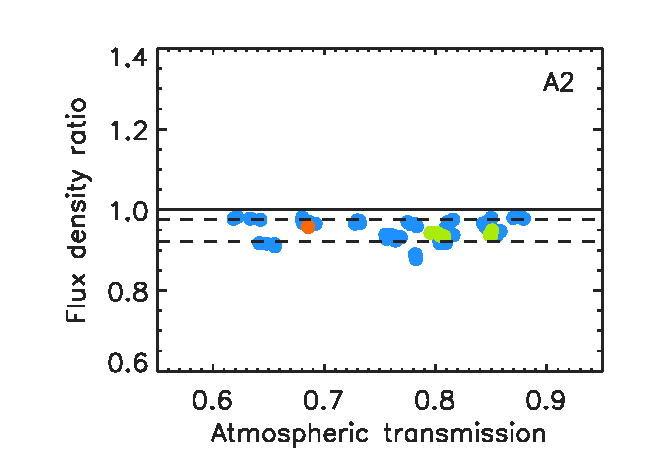
\includegraphics[clip=true, trim={1.8cm, 0.2cm, 0.5cm, 0.7cm},width=0.457\linewidth]{Figures/plot_flux_density_ratio_MWC349_obstau_corrected_skydip_narrow_a2.pdf}
    \begin{overpic}[clip=true, trim={0.9cm, 0.2cm, 0, 0.6cm},width=0.532\linewidth]{Figures/plot_flux_density_ratio_MWC349_obstau_tau225_narrow_1mm.pdf}
      \put(20,60){\footnotesize {\tt Taumeter}}
    \end{overpic}
    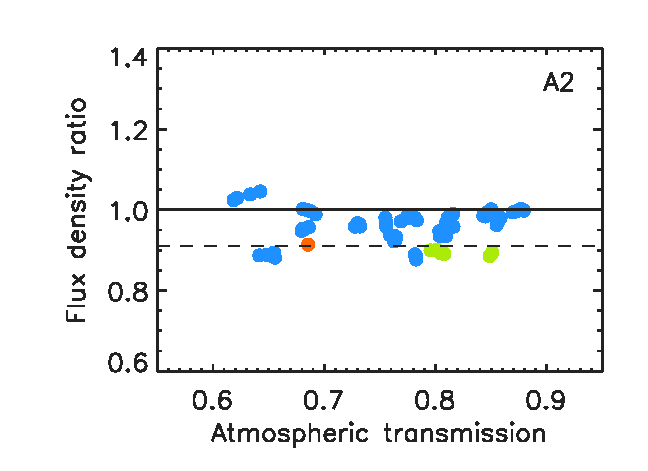
\includegraphics[clip=true, trim={1.8cm, 0.2cm, 0.5cm, 0.7cm},width=0.457\linewidth]{Figures/plot_flux_density_ratio_MWC349_obstau_tau225_narrow_a2.pdf}
    \begin{overpic}[clip=true, trim={0.9cm, 0.2cm, 0, 0.6cm},width=0.532\linewidth]{Figures/plot_flux_density_ratio_MWC349_obstau_skydip_narrow_1mm.pdf}
      \put(20,60){\footnotesize {\tt Skydip}}
    \end{overpic}
    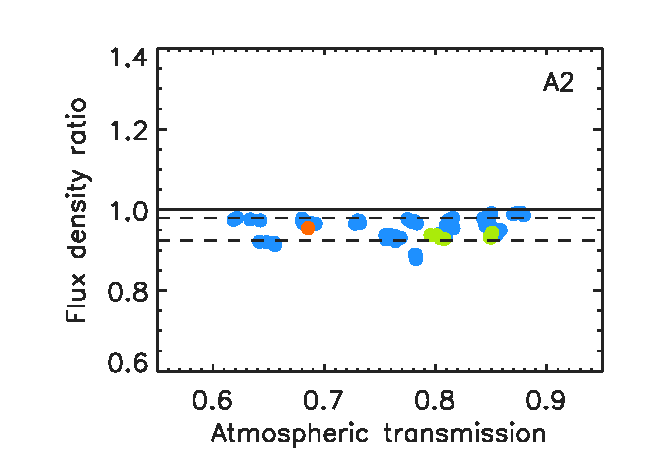
\includegraphics[clip=true, trim={1.8cm, 0.2cm, 0.5cm, 0.7cm},width=0.457\linewidth]{Figures/plot_flux_density_ratio_MWC349_obstau_skydip_narrow_a2.pdf}
    \begin{overpic}[clip=true, trim={0.9cm, 0.2cm, 0, 0.6cm},width=0.532\linewidth]{Figures/plot_flux_density_ratio_MWC349_obstau_corrected_skydip_photocorr_demo_narrow_1mm.pdf}
      \put(20,60){\footnotesize {\tt PC-demo}}
    \end{overpic}
    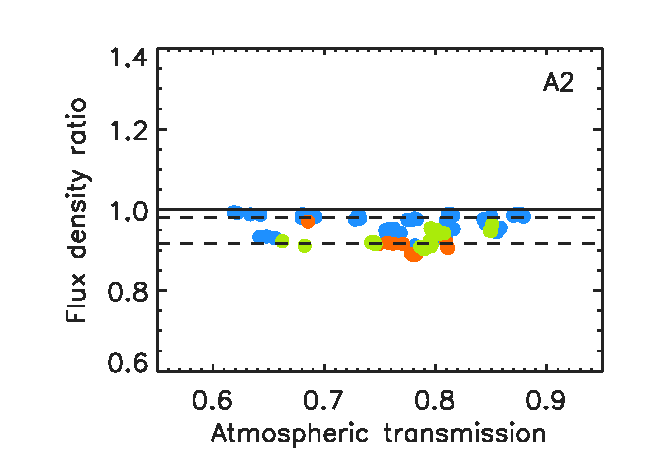
\includegraphics[clip=true, trim={1.8cm, 0.2cm, 0.5cm, 0.7cm},width=0.457\linewidth]{Figures/plot_flux_density_ratio_MWC349_obstau_corrected_skydip_photocorr_demo_narrow_a2.pdf}
    \begin{overpic}[clip=true, trim={0.9cm, 0.4cm, 0, 0.6cm},width=0.532\linewidth]{Figures/plot_flux_density_ratio_MWC349_obstau_corrected_skydip_photocorr_pointing_narrow_1mm.pdf}
      \put(20,60){\footnotesize {\tt PC-point}}
    \end{overpic}
    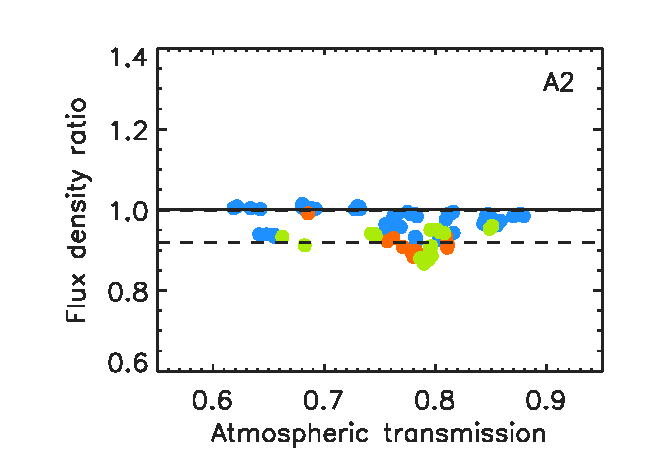
\includegraphics[clip=true, trim={1.8cm, 0.4cm, 0.5cm, 0.7cm},width=0.457\linewidth]{Figures/plot_flux_density_ratio_MWC349_obstau_corrected_skydip_photocorr_pointing_narrow_a2.pdf}
    \vspace{-0.3cm}
    \caption[Calibration bias comparison]{Comparison of the
        calibration bias for five calibration methods using
          observations of MWC349.
       The measured-to-expected flux density ratio is shown as a
      function of the atmospheric transmission for the baseline method
      (first row) as well as for methods using the {\tt taumeter} (second
      row) and {\tt skydip} (third) opacity correction, and for methods
      resorting to the {\tt PC-demo} (fourth) and {\tt PC-point} (fifth)
      photometric corrections. Dashed lines
      show the flux density ratio rms errors.}
    \label{fig:mwc349_obstau_others}
  \end{center}
\end{figure}
%
Table~\ref{tab:baseline-photometry} gathers the calibration bias
estimates for the three observation campaigns and for all the scans.
In the $1\,\rm{mm}$ band, we find
$b_\nu$ in agreement with unity within the statistical dispersion for
the three campaigns,
whereas a $5\%$ lack of flux with respect to expectations is observed
at $2\,\rm{mm}$, consistently for the three campaigns. This bias has a
low significance with respect to the absolute calibration precision of
NIKA2 (see Sect.~\ref{se:photometry_criteria}).
%{\lp Furthermore, the flux density expectations have also
%uncertainties.}
%and PdBI, which depend on the precicision with which the
%primary calibrator flux densities are known. For Uranus, the model
%uncertainties are of about $5\%$, as reported
%in~\citet{Morenothesis,Bendo2013}. 
This will be further investigated by using other calibration methods
in Sect.~\ref{se:photometry_others}.

%  BASELINE RESULTS
%%%%%%%%%%%%%%%%%%%%%%%%%%%%%%%%%%%%%%%%%%%%%%%%%%%%%%%%%%%%%%%%%%
\begin{table}[!thbp]
  \begin{center}
    \caption[Baseline calibration results]{Baseline calibration results:
  photometry accuracy and uncertainties. The first sub-panel labelled 'Bias' gives the
  calibration bias $b_{\nu}$ and the second sub-panel labelled 'Rms' the calibration
  rms error $\sigma_{\nu}$, as defined in
  Sect.~\ref{se:photometry_criteria},
  using observations during N2R9, N2R12, N2R14 and the combination of
  the three campaigns. {\lp In each sub-panel, the first row indicates the
    number of acquired scans, while the second row gives the
    number of selected scans using the \emph{baseline} scan selection.}}
\label{tab:baseline-photometry}
\begin{tabular}{clrrrr}
  \hline\hline
  \noalign{\smallskip}
 % \multicolumn{2}{c}{}  &  \multicolumn{4}{|c}{Datasets}  \\\cline{3-6}
  \multicolumn{2}{c}{Characteristics} &  N2R9  & N2R12   &  N2R14 & Combined \\
  \noalign{\smallskip}
  \hline
  \noalign{\smallskip}
%  Bias &  $\#$ total    &  68    &  14     &   27     &    109    \\
%       &  $\#$ selected &  64    &   1     &   7      &     72    \\
%       &  A1            &  0.99  &  1.06   &   0.98   &   0.98    \\
%       &  A3            &  1.01  &  1.08   &   1.04   &   1.00    \\
%       &  1mm           &  1.00  &  1.07   &   1.01   &   0.99    \\
%       &  2mm           &  0.95  &  0.96   &   0.94   &   0.95    \\
%  \hline
%  \multicolumn{6}{|l|}{using colour corrections as of Table A.1}  \\
%  \hline
  Bias &  $\#$ total    &  68    &  14     &   27     &    109    \\
       &  $\#$ selected &  64    &   1     &   7      &     72    \\
       &  A1            &  0.95  &  1.03   &   0.94   &   0.95    \\
       &  A3            &  0.99  &  1.07   &   1.00   &   1.00    \\
       &  1mm           &  0.97  &  1.05   &   0.97   &   0.98    \\
       &  2mm           &  0.95  &  0.95   &   0.93   &   0.95    \\
  \hline
  \noalign{\smallskip}
  Rms  &  $\#$ total    &  303   &  72     &   112    &    487   \\
  $[\%]$ &  $\#$ selected &  219   &  33     &    12    &    264   \\
       &  A1            &  5.7   &  4.6    &   2.9    &    5.5   \\
       &  A3            &  6.2   &  5.7    &   2.4    &    6.0   \\
       &  1mm           &  5.9   &  5.0    &   2.5    &    5.7   \\
       &  2mm           &  3.2   &  2.1    &   1.1    &    3.0   \\  
\hline
\end{tabular}
\end{center}
\end{table}
%The baseline calibration relative uncertaintes, as defined in
%Sect.~\ref{se:photometry_criteria}, are evaluated using bright
%sources. From a total of 487 scans
%flux-selected sources acquired during N2R9, N2R12 and N2R14, 264 met
%the baseline selection criteria and are used for testing stability.

\begin{figure}[!thbp]
  \begin{center}
%    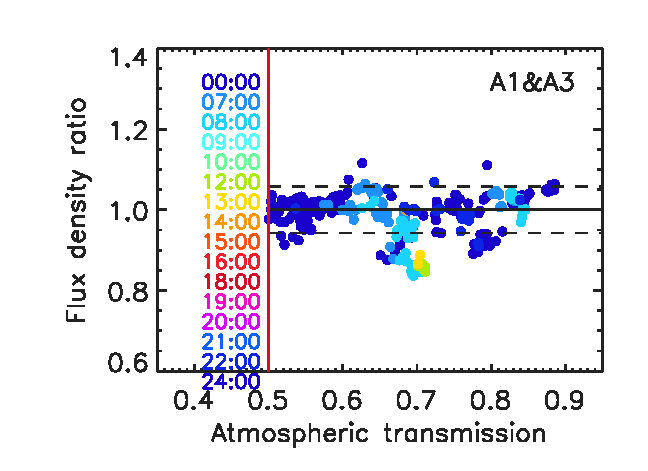
\includegraphics[clip=true, trim={0.9cm, 0.2cm, 0, 0.7cm},width=0.532\linewidth]{Figures/plot_flux_density_ratio_obstau_allbright_obsdate_corrected_skydip_narrow_1mm.pdf}
%    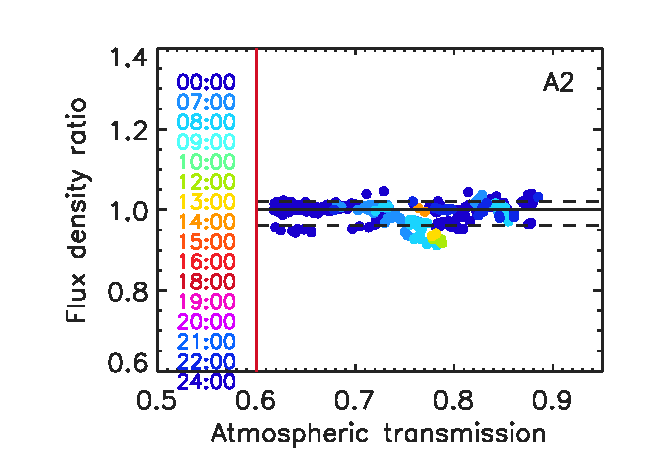
\includegraphics[clip=true, trim={1.8cm, 0.2cm, 0.5cm, 0.7cm},width=0.455\linewidth]{Figures/plot_flux_density_ratio_obstau_allbright_obsdate_corrected_skydip_narrow_a2.pdf}
%    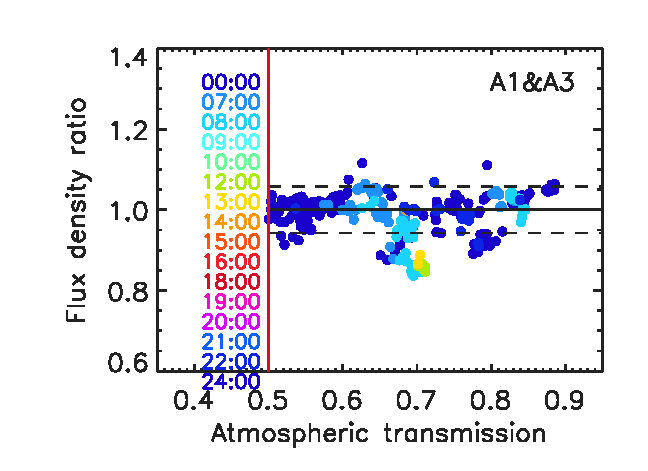
\includegraphics[clip=true, trim={0.9cm, 0.2cm, 0.5cm, 0.7cm},width=0.65\linewidth]{Figures/plot_flux_density_ratio_obstau_allbright_obsdate_corrected_skydip_narrow_1mm.pdf}
%     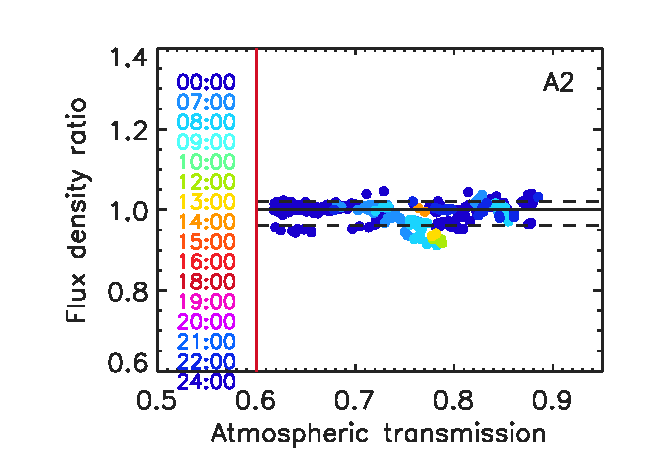
\includegraphics[clip=true, trim={0.9cm, 0.2cm, 0.5cm, 0.7cm},width=0.65\linewidth]{Figures/plot_flux_density_ratio_obstau_allbright_obsdate_corrected_skydip_narrow_a2.pdf}
      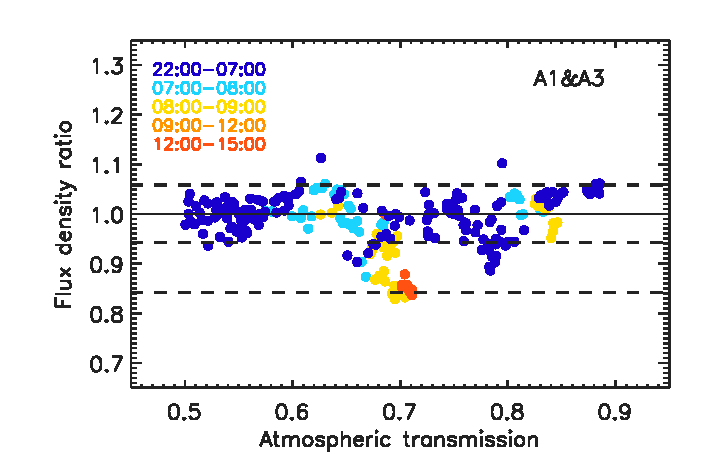
\includegraphics[clip=true, trim={0.9cm, 0, 0.5cm, 0.6cm},width=0.75\linewidth]{Figures/plot_flux_density_ratio_obstau_allbright_obsdate_corrected_skydip_rescaled_1mm.pdf}
     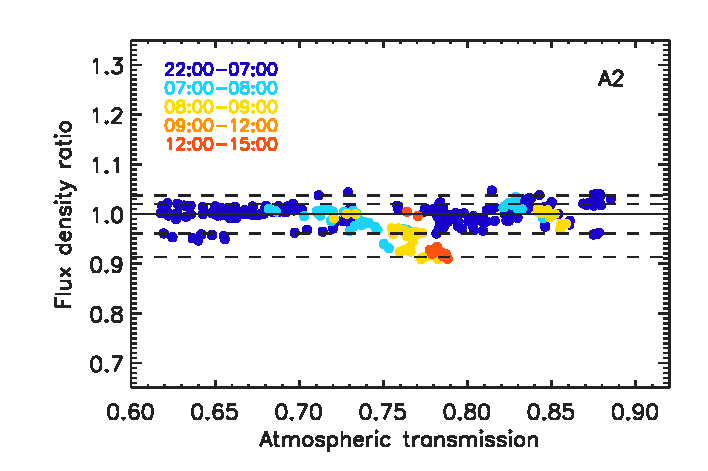
\includegraphics[clip=true, trim={0.9cm, 0, 0.5cm, 0.6cm},width=0.75\linewidth]{Figures/plot_flux_density_ratio_obstau_allbright_obsdate_corrected_skydip_rescaled_a2.pdf} 
    \caption[Baseline calibration rms error estimate]{Baseline
      rms calibration uncertainties. The
      measured-to-median flux density ratio of bright sources is
      plotted as a function of the atmospheric transmission
      colour-coded according to the UT
      observation time of the scans for the combination of A1$\&$A3
      (top panel)
      and for A2 (bottom panel).
      The inner dashed lines from either sides of the
      unity-ratio line show the rms errors, {\lp which
      are less than 6\% at $1\,\rm{mm}$ and 3\% at $2\,\rm{mm}$, while
      the outer dashed lines show the $95\%$ confidence level contours.}
      The lowest flux ratio data points correspond to some of the
      scans acquired during daytime between 8:00 UT and 15:00 UT
      hours (yellow and red), while the scans acquired during night-time
      between 22:00 UT and 7:00 UT yield data points (dark blue)
      well distributed within the rms error with a few outliers.}
    \label{fig:allbright_rms_corrected_skydip}
  \end{center}
\end{figure}
Figure~\ref{fig:allbright_rms_corrected_skydip} shows the
measured-to-median flux densities evaluated from bright source scans
for the combination of Array $1\&3$ and Array 2 as a function of the
atmospheric transmission and colour-coded as a function of the
observation time. From a total of 487 scans towards
flux-selected sources, acquired during N2R9, N2R12 and N2R14, 264 met
the baseline selection criteria and are included in
Fig.~\ref{fig:allbright_rms_corrected_skydip} for testing the
calibration stability. The calibration uncertainties are
estimated using the standard deviation of the flux density ratios for
the three campaigns. Results are gathered in
Table~\ref{tab:baseline-photometry}.
Combining all the scans, we find rms uncertainties of $5.5\%$ for A1,
$6.0\%$ for A3, $5.7\%$ for the $1\,\rm{mm}$ band and $3.0\%$ for A2.
%%%%%%% 95% %%%%%%%%%%%%%%%%%%%%%%%%
{\lp Using the flux ratio distributions, we construct the 68 and 95\%
C.L. intervals. The 68\% C.L. intervals are $-6.4\%$ and $+3.4\%$ at
$1\,\rm{mm}$ and $-3.8\%$ and $+1.5\%$ at $2\, \rm{mm}$. Hence in average
the 68\% C. L. errors are of $4.9\%$ and $2.7\%$ at 1 and $2\, \rm{mm}$,
respectively. We conclude that the rms errors are conservative
estimates of the 68\% C. L. errors at both wavelengths. The 95\%
C.L. contours are $-15.8\%$ and $+5.9\%$ at $1\,\rm{mm}$ and $-8.6\%$ and
$+3.8\%$ at $2\, \rm{mm}$.
The rms errors and the 95\%
C.L. interval are shown in
Fig.~\ref{fig:allbright_rms_corrected_skydip} with the inner and
outer dashed lines, respectively.} 

The flux density ratio is constant within the rms errors along the
wide range of tested atmospheric transmission, ranging from 0.5 to 0.9
at $1\,\rm{mm}$.
However, some scans at atmospheric transmissions of about 0.7 at
$1\,\rm{mm}$ show a mild lack of flux density with respect to the
median within the 95\% C. L. contours. The scans
affected by the lack of flux have all been observed
either between 12:00 and 14:00 UT or between 8:00 and 9:00 UT,
that are close to the threshold of the observation time cuts of
the \emph{baseline} scan selection (see
Sect.~\ref{se:data_selection}). These scans are likely
to be affected by the \afternoon\ beam broadening or by the
sunrise focus drift, respectively. Furthermore, we find that restricting the
used observation time to the 10 more stable hours (from 22:00 to
08:00 UT) would result in rms calibration uncertainties of
$3.6\%$ at $1\,\rm{mm}$ and $1.2\%$ at $2\,\rm{mm}$, which constitute an
improvement of about $60\%$ at $1\,\rm{mm}$ and $40\%$ at $2\,\rm{mm}$
of the rms errors.  
The \emph{baseline} scan selection, which i)
retains 16 hours of observation time
a day and ii) %results in calibration uncertainties that meet the
%requirement for a millimetric ground-based instrument,
{\lp results in state-of-the-art rms calibration
uncertainties,} constitutes {\lp an useful trade-off representative of most
of the observations with NIKA2.} 

%---------------------------------------------------------------------
%
%	Comparaison
%
%---------------------------------------------------------------------
\subsection{Comparison with other calibration methods}
\label{se:photometry_others}
% ALL METHOD RESULTS 
\begin{table*}[!htbp]
\begin{center}
\caption[Comparison of calibration results using five
  methods]{Comparison of results using five calibration
  methods: (first column) the \emph{baseline} calibration, (second and
  third) the calibration methods using other opacity correction, {\tt
  taumeter} and {\tt skydip}, respectively, and
  (fourth and fifth) the calibration methods using a photometric correction, {\tt
  PC-demo} and {PC-point}, respectively (see Appendix~\ref{se:photometric_correction}).  
  The calibration biases, as defined in
  Sect.~\ref{se:def_calibration_bias}, are reported in the sub-panel
  labelled 'Bias'. The sub-panel labelled 'Rms' gathers (first row) the total number of
  observation scans of bright sources (see
  Sect.~\ref{se:def_calibration_rms_error}) acquired during
  the \emph{reference} campaigns, (second row) the number of selected
  scans, and (third to sixth rows) the rms calibration uncertainties
  (Sect.~\ref{se:def_calibration_rms_error}) for Array 1, Array 3, the
  combination of A1 and A3, and Array 2, respectively. }
\label{tab:Calibration_results_all}
\begin{tabular}{clrrrrr}
  \hline\hline
  \noalign{\smallskip}
  \multicolumn{2}{c}{}  &  \multicolumn{5}{c}{Methods} \\\cline{3-7}
  \noalign{\smallskip}
  \multicolumn{2}{c}{Characteristics} &  baseline  & {\small {\tt taumeter}}  & {\small {\tt skydip}}  &  {\small {\tt PC-demo}} & {\small {\tt PC-point}} \\
  \hline
  \noalign{\smallskip}
  %Bias &  $\#$ total    &   109   &   109    &   109    &    109    &  109   \\
  %     &  $\#$ selected &    72   &   72     &    72    &     96    &   95   \\
  %     &  A1            &   0.98  &  1.01    &  0.99    &   0.98    &  1.00  \\
  %     &  A3            &   1.00  &  1.04    &  1.01    &   1.01    &  1.02  \\
  %     &  1mm           &   1.00  &  1.03    &  1.00    &   1.00    &  1.01  \\
  %     &  2mm           &   0.95  &  0.96    &  0.95    &   0.95    &  0.95  \\
  %\hline
  %\multicolumn{7}{|l|}{Using colour corrections as of Table A.1} \\
  %\hline
  Bias &  A1            &   0.95   &  0.98    &  0.97    &   0.95    &  0.97  \\
       &  A3            &   1.00   &  1.02    &  1.02    &   0.99    &  1.00  \\
       &  1mm           &   0.98   &  1.01    &  1.00    &   0.97    &  0.99  \\
       &  2mm           &   0.95   &  0.95    &  0.95    &   0.95    &  0.95  \\
  \hline
  \noalign{\smallskip}
  Rms  &  $\#$ total      &   487    &    487   &    487    &    396    &  396 \\
  $[\%]$ &  $\#$ selected &   264    &    264   &    264    &    291    &  283 \\
       &  A1            &   5.5    &    7.5   &    7.3    &    4.0    &  4.9 \\
       &  A3            &   6.0    &    8.1   &    7.1    &    4.1    &  5.2 \\
       &  1mm           &   5.7    &    7.9   &    7.1    &    3.8    &  4.9 \\
       &  2mm           &   3.0    &    3.8   &    3.0    &    2.2    &  2.4 \\
\hline
\end{tabular}
\end{center}
\end{table*}

In this section, the \emph{baseline} calibration results are compared to
results drawn either using other calibration methods obtained from different
opacity corrections ({\tt taumeter} and {\tt skydip} as
discussed in Sect.~\ref{se:baseline_calibration_opacity}), or
including a photometric correction ({\tt PC-demo} and {\tt PC-point},
as described in Appendix~\ref{se:photometric_correction}) to mitigate
the \afternoon\ variation effect (Sect.~\ref{se:beam_variation}).
For robustness test, we evaluate and compare the photometry quality criteria of
Sect.~\ref{se:photometry_criteria} for the five calibration methods.


\subsubsection{Calibration bias}
\label{se:calibration_bias_all}

We present the calibration bias as a function of the atmospheric
transmission for the five calibration methods in
Fig.~\ref{fig:mwc349_obstau_others} and report the results in the row
labelled 'Bias' of Table~\ref{tab:Calibration_results_all}.

At $1\,\rm{mm}$, all methods lead to flux density estimates in
agreement with expectations within the rms dispersion. However,
{\tt taumeter} flux ratios have more dispersion than
the \emph{baseline} flux ratios whereas {\tt skydip} shows some
dependency on the atmospheric
transmission, with a 10 to $15\%$ excess of the flux density with
respect to expectations at high transmission. This residual
systematic effect has motivated the development of the {\tt corrected
  skydip} method, as discussed in
Sect.~\ref{se:corrected-skydip}. These features, which are
already noticeable from Fig.~\ref{fig:mwc349_obstau_others}, will be
confirmed and further discussed later using more observation scans. On
the other hand, the calibration methods based on photometric
correction (Appendix~\ref{se:photometric_correction}) yield an
unbiased photometry (calibration bias in agreement with unity
within the rms error) while allowing the use of $30\%$ more
scans. These results are encouraging for the exploitation of scans
acquired during the observing periods
impacted by the \afternoon\ beam variation effect
(Sect.~\ref{se:beam_variation}).

At $2\,\rm{mm}$, all methods result in a similar calibration bias
of $0.95$ with a rms error of $0.05$ estimated on the MWC349 scans. 
This corresponds to a low-significance $5\%$ lack of flux density
towards MWC349.
%We also obtained the same calibration
%biases for each observation campaign (see
%Table~\ref{tab:baseline-photometry}).
To summarize, the calibration bias at $2\, \rm{mm}$ is stable against
i) a large range of atmospheric conditions, ii) the observation campaign, iii) the
opacity correction method, iv) the method to treat the
temperature-induced beam variation effect.
%An explanation for the
%$5\%$ lack of flux density towards
%MWC349 is probably to be seeked on the side of the flux density
%expectations for this source.
This $5\%$ lack of flux density is thus probably due to
uncertainties on the flux density expectations for this source.
They come in two flavours.
{\lp Firstly the uncertainties on the flux expectation, as reported in
Appendix~\ref{se:ref_flux_secondaries}, consist in the propagation of
the errors on the fitted SED from the \emph{Plateau de Bure Interferometre}
(PdBI) and the \emph{Very Large Array} (VLA) observations. Systematic
uncertainties that may also impact the SED are not included.}  
%the accuracy of the SED fitted from PdBI and VLA observations
%(see Sect.~\ref{se:ref_flux_secondaries})
%depends on these instruments absolute flux density calibration, which
%is at least greater than the $5\%$ primary calibrator model accuracy,
Secondly, the NIKA2 flux density extrapolation from
interferometer data may be not straightforward for MWC349. {\lp In
particular, NIKA2 flux extrapolation ignores the contamination by
strong masers in the radio recombination lines~\citep{masingRRL},
while strong maser emission lines are masked in PdBI observations to
measure the continuum. In addition, the resulting continuum shows
indications of variability.}


\subsubsection{Calibration rms uncertainties}

The calibration rms uncertainties for the five methods evaluated using
flux-selected source scans are gathered in the sub-panel labelled 'Rms'
of Table~\ref{tab:Calibration_results_all}.

Compared to the \emph{baseline} method, the {\tt taumeter} method leads to 
rms errors increased of about $40$ and $30\%$ at 1 and
$2\,\rm{mm}$, respectively. The {\tt skydip} method shows lower
dispersion but a mild correlation with the atmospheric transmission, as
discussed in Sect.~\ref{se:calibration_bias_all}.

In addition, we have checked the flux density ratios for the bunch of
scans with an atmospheric transmission of about 0.7, which were
discussed in Sect.~\ref{se:photometry_baseline}, by comparing
calibration methods with or without photometric correction. The
flux density ratios are low (within the 95\% C.L. interval) for the scans
observed within 12:00 and 15:00 UT in the three first methods, as shown in
Fig.~\ref{fig:allbright_rms_corrected_skydip} for
the \emph{baseline} method. By contrast, they are within the 68\% C.L. interval
when using a photometric correction. This further validates the
hypothesis that the low flux
density of these scans is due to \afternoon\ beam effect, as assumed in
Sect.~\ref{se:photometry_baseline}. This also constitutes an example
of the calibration improvement obtained by using a
photometric correction.

Moreover, results based on the {\tt PC-demo} method show that rms
calibration uncertainties as low as $3.8$ and $2.2\%$
at 1 and $2\,\rm{mm}$ are within the reach of NIKA2 {\lp without any
selection based on the observation time.}
%without rejecting any observations.
However, we recall this method relies on 
accurate beam estimates. Using {\tt PC-point}, which is the
practical case, still improves the calibration uncertainties
w.r.t. the \emph{baseline} results but by a factor of about $20\%$ in both
bands. Furthermore, the differences between
the flux density ratios from {\tt PC-demo} and {\tt PC-point}, which are
seen e.g. from the corresponding panels of
Fig.~\ref{fig:mwc349_obstau_others}, are likely
to be due to the photometric correction noise
when monitoring the beam from pointing scans (see
Appendix~\ref{ap:beam_monitoring}). We conclude that more
control on the beam monitoring is needed before routinely using a calibration
based on photometry correction. By contrast, the baseline method
combines good performance with robustness.


\subsection{Summary}
\label{se:photometry_summary}
Among the methods that rely on the UT hour-based
scan selection to mitigate the effect of beam size variations, the
\emph{baseline} method shows the best performance in terms of calibration
bias and uncertainties. The methods that rely on a photometric correction
show good calibration results, and thus represent a promising lead
to further improve the calibration uncertainties. However, their
robustness depends on the accuracy of the beam monitoring. {\lp The
proposed beam monitoring based on {\tt pointing} scans induces some
extra dispersion of the flux densities. A more accurate beam monitoring is
feasible but requires using dedicated observation scans.} 
From the \emph{baseline} method results discussed in
Sect.~\ref{se:photometry_baseline}, we have found that the measured
flux density of MWC349 is in agreement with expectations within $5\%$
for both wavelengths. Moreover, the {\rev point-source} rms calibration
uncertainties are of $5.7\%$ at $1\,\rm{mm}$ and of $3\%$ at $2\,\rm{mm}$
using a series of 264 scans of sources of flux density above
$1\, \rm{Jy}$.
These results demonstrate the excellent accuracy and stability of the
NIKA2 {\rev point-source} photometric capabilities.





